\documentclass[12pt]{article}
\usepackage{graphicx} % This lets you include figures
\usepackage{hyperref} % This lets you make links to web locations
\graphicspath{ {./images/} }

\usepackage[rightcaption]{sidecap}
\usepackage{caption}
\usepackage{subcaption}
\usepackage{hyperref}

\usepackage{float}

\usepackage{imakeidx}

\usepackage{tikz}
\usetikzlibrary{shapes.geometric, arrows}
\tikzstyle{startstop} = [rectangle, rounded corners, minimum width=3cm, minimum height=1cm,text centered, draw=black, fill=red!30]
\tikzstyle{io} = [trapezium, trapezium left angle=70, trapezium right angle=110, minimum width=3cm, minimum height=1cm, text centered, draw=black, fill=blue!30]
\tikzstyle{process} = [rectangle, minimum width=3cm, minimum height=1cm, text centered, draw=black, fill=orange!30]
\tikzstyle{decision} = [diamond, minimum width=3cm, minimum height=1cm, text centered, draw=black, fill=green!30]
\tikzstyle{arrow} = [thick,->,>=stealth]

\usepackage{todonotes}

\usepackage{amsmath,amssymb}
\let\amssymbboxplus\boxplus
\let\amssymbboxminus\boxminus

\renewcommand{\boxplus}{\mathbin{\mathop\amssymbboxplus}}
\renewcommand{\boxminus}{\mathbin{\mathop\amssymbboxminus}}

\usepackage[noend]{algpseudocode}


\makeindex


\title{Computer and network security}
\author{Beau De Clercq}
\date{2020-2021}

\begin{document}
	
 \maketitle{}
 
 \tableofcontents
 
 \clearpage
 \newpage
 
 \section{Introduction}
 
 \section{Symmetric ciphers}
 
 \newpage
 \section{Message authentication}
 \subsection{Hash functions}
 A hash function H is a function that takes input data blocks of length M and returns a hash value of fixed size R.\\
 A cryptographic hash function that also satisfies following conditions:
 \begin{itemize}
 	\item One way property: it should be infeasible to find a data object that maps to a predefined hash value.
 	\item Collision free property: it should be infeasible to find 2 data objects that map to the same hash value.
 	\item Use padding to pad up input to fixed length and add the length l of the block in bits. 
 \end{itemize}
By satisfying the first two properties, hash functions can  be used to determine if data has been altered.
\subsubsection{Applications}
Hash functions can be used in an number of applications:
\begin{itemize}
	\item Message authentication: to ensure a message hasn't been altered.
	\item Digital signatures: ensure the authenticity of messages and identity of the sender.
	\item One-way password file: store hash value of password in plain text file.
	\item Intrusion/virus detection: store H(f) for each file to determine if files have been modified.
	\item Pseudorandom function: use H to generate pseudorandom private key.
\end{itemize}
\subsubsection{Security requirements}
Cryptographic hash functions must adhere to following security requirements:
\begin{itemize}
	\item Basic:
	\begin{itemize}
		\item Input data can be of any size
		\item Output is of fixed length
		\item H(x) is easy to compute
	\end{itemize}
	\item Advanced:
	\begin{itemize}
		\item Given h, it is hard to find y: H(y) = h
		\item It is hard to find y: y$\ne$x $\&$ H(y)=H(x)
		\item It is hard to find (x, y): H(x)=H(y)
	\end{itemize}
\end{itemize}

\subsubsection{Attacks}
\begin{itemize}
	\item \underline{Brute force preimage attack}\\
	The goal of this attack is to find a y such that H(y) = h for a given hash value h.\\
	The attack itself goes as follows:\\
	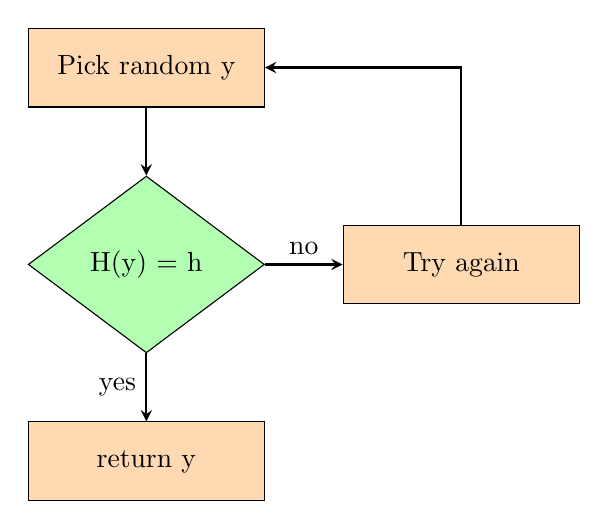
\begin{tikzpicture}[node distance=2cm]
	
	\node (pro1) [process] {Pick random y};
	\node (dec1) [decision, below of=pro1, yshift=-0.5cm] {H(y) = h};
	\node (pro2a) [process, below of=dec1, yshift=-0.5cm] {return y};
	\node (pro2b) [process, right of=dec1, xshift=2cm] {Try again};

	\draw [arrow] (pro1) -- (dec1);
	\draw [arrow] (dec1) -- node[anchor=east] {yes} (pro2a);
	\draw [arrow] (dec1) -- node[anchor=south] {no} (pro2b);
	\draw [arrow] (pro2b) |- (pro1);

	\end{tikzpicture}\\
	On average this attack need $2^{m-1}$ attempts for an m-bit hash value.
	\item \underline{Brute force collision resistance attack}\\
	The goal of this attack is to find two values x and y such that H(x) = H(y). This attack needs $2^{\frac{m}{2}}$ attempts for an m-bit hash value.\\
	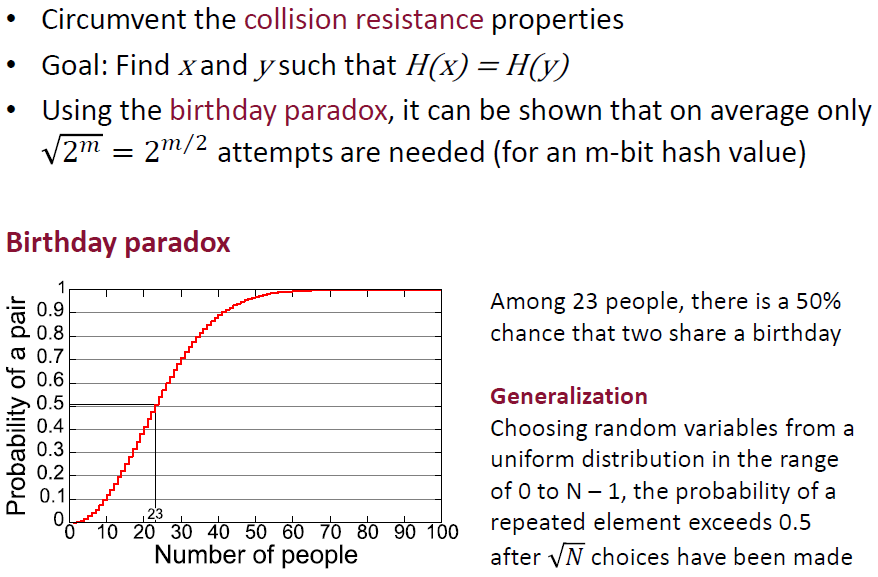
\includegraphics[width=\linewidth]{./slides/L3P1BFCOL.PNG}
\end{itemize}
 
 \subsection{Secure Hash Algorithm (SHA)}
 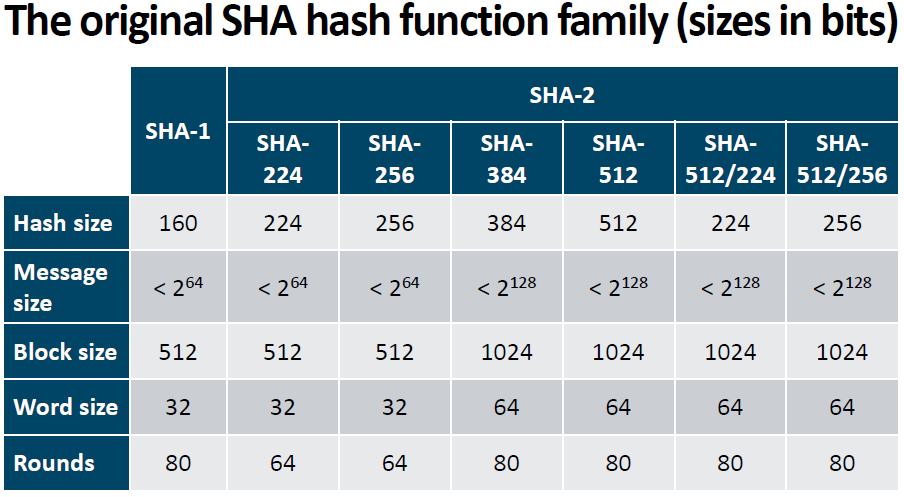
\includegraphics[width=0.8\linewidth]{./slides/L3P2SHA.PNG}
 \subsubsection{SHA512}
 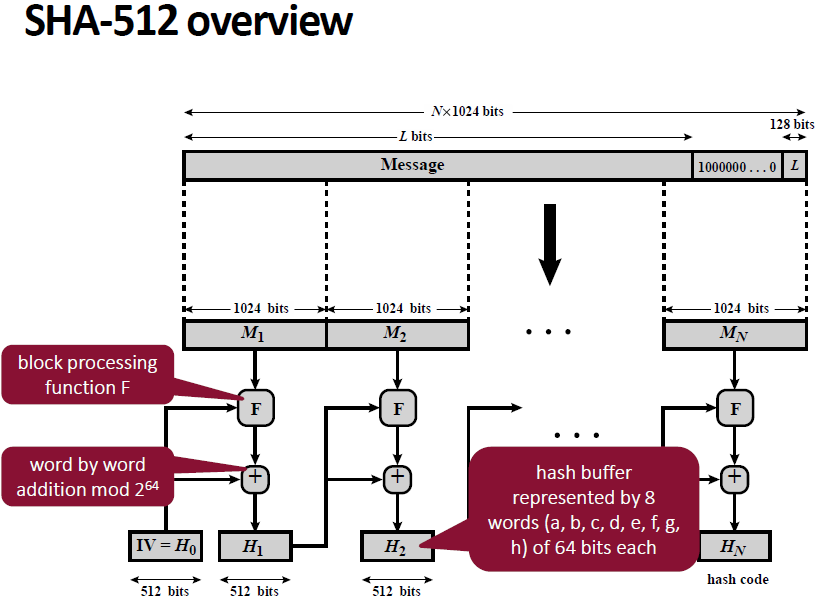
\includegraphics[width=\linewidth]{./slides/L3P2SHA512.PNG}
 \subsubsection{SHA512 block processing}
 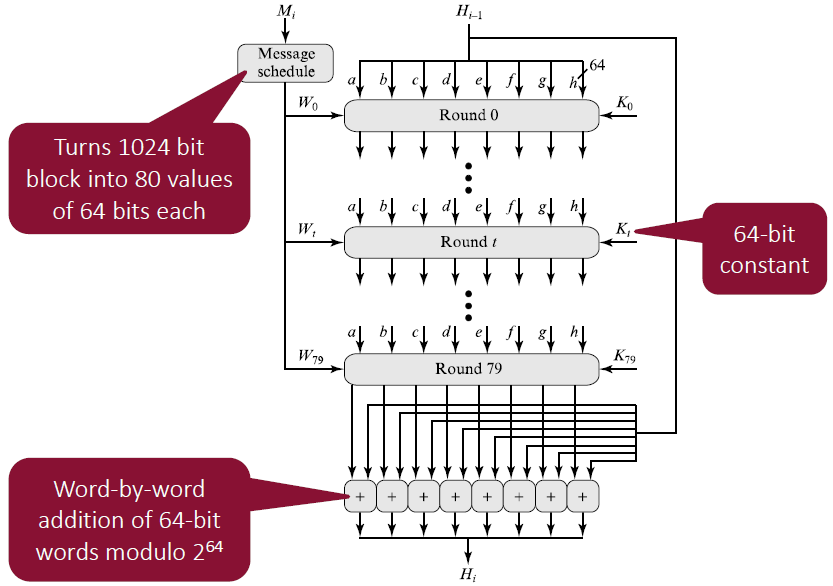
\includegraphics[width=0.8\linewidth]{./slides/L3P2SHA512BLOCK.PNG}\\
 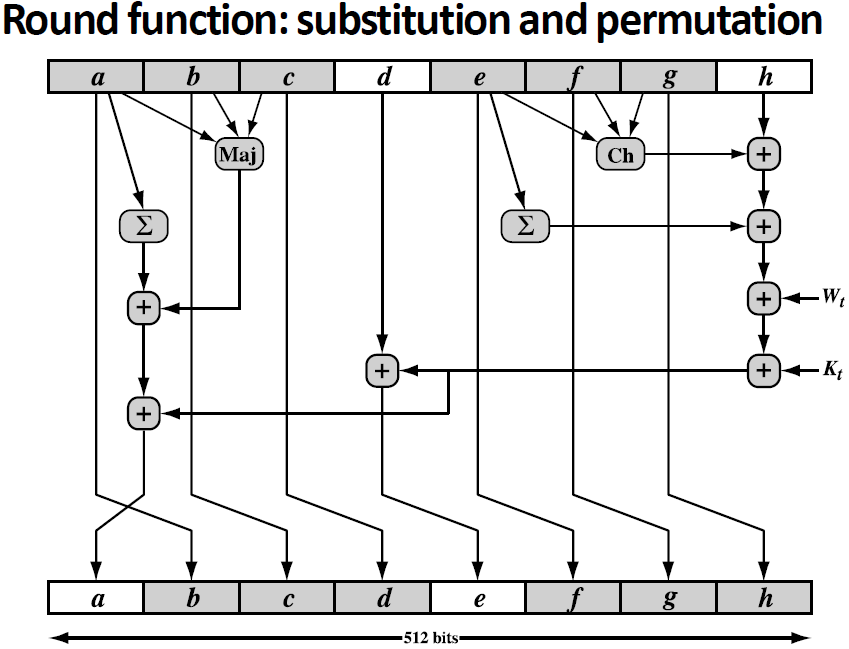
\includegraphics[width=0.8\linewidth]{./slides/L3P2SHA512ROUND.PNG}
 In this 80 round process, a message of 1024 bits is transformed into 80 values of 64 bits each which are then individually processed in sequence by means of a round function.\\
 After the final round a word-by-word addition 64-bit words mod$2^{64}$ is performed to obtain the final hashed value.
 \subsubsection{Message schedule}
 The first 16 words $W_0 .. W_{15}$ are derived directly from the input block $M_i$. All other words are derived as follows:
 \begin{align*}
 	W_t = W_{t-16} \boxplus \delta_0(W_{t-15}) \boxplus W_{t-7} \boxplus \delta_1(W_{t-2})\\
 	\delta_0(x) = ROTR^1(x) \oplus ROTR^8(x) \oplus SHR^7(x)\\
 	\delta_1(x) = ROTR^{19}(x) \oplus ROTR^{61}(x) \oplus SHR^6(x)\\
 	ROTR^n(x) = \text{circular right bit-shift by n bits}\\
 	SHR^n(x) = \text{right bit-shift of x by n bits with}\\
 	 \text{padding by n zeros on the left}
 \end{align*}
 
 \subsection{Length extension attack and SHA3}
 \subsubsection{Length extension attack}
 Type of attack where an attacker can use H($M_1$) and the length of $M_1$ to calculate H($M_1|M_2$) for an attack controlled message $M_2$ without needing to know the content of $M_1$. This is done by taking the old message and using it as 'intermediary' input in the hashing algorithm.
 \subsubsection{SHA3}
 \todo[inline]{Add image from slides}
 
 \subsection{Message authentication}
 There are 8 types of attacks:
 \begin{enumerate}
 	\begin{multicols}{2}
 		\item Disclosure of message content
 		\item Traffic analysis
 		\item Masquerade
 		\item Content modification
 		\item Sequence modification
 		\item Timing modification
 		\item Source repudiation
 		\item Destination repudiation
 	\end{multicols}
 \end{enumerate}
 Items 1 and 2 can be countered using confidentiality mechanisms, eg symmetric encryption.\\
 Items 3 to 6 can be countered by using \underline{message authentication} to verify that the received message hasn't been altered.\\
 \underline{Digital signatures} can be seen as an extension to message authentication as it is an authentication technique that also includes measures to counter repudiation by the source.\\
 \newline
 A message authentication function is a function that produces an authenticator (a value to be used to authenticate a message). There are 3 classes of message authentication functions:
 \begin{itemize}
 	\item Hash functions:
 	\begin{itemize}
 		\item Concatenate message M with secret key S and hash the stream
 		\item Send message M together with hash value: if it is intercepted an attacker can't create a new hash value since the key is unknown
 		\item Check authentication: combine M with S, hash the stream and compare with received hash value
 	\end{itemize}
 	\item Message encryption, eg using symmetric encryption, provides both confidentiality and authentication if key K is secret. If the decrypted message M is not meaningful then the message can be considered altered.
 	\item Message authentication code (MAC): generates fixed-size cryptographic checksum based on message and secret key
 	\begin{itemize}
 		\item Does not need to be reversible
 		\item send message with checksum: if the checksum calculated by the receiver doesn't match then the message has been altered
 		\item Cannot be used to provide digital signatures: a signature need to be verifiable by anyone and MAC requires the use of a secret key
 	\end{itemize}
 \end{itemize}
 \subsubsection{Security requirements for MAC}
 \begin{itemize}
 	\item If an opponent observes $M$ and $MAC(K, M)$, it should be infeasable to construct $M'$ such that $MAC(K, M') == MAC(K, M)$.
 	\item Given 2 randomly chosen messages $M$ and $M'$, the probability that $MAC(K, M) == MAC(K, M')$ should be $2^{-N}$ for an N-bit code. $-->$ codes should be distributed uniformly and random over the entire output space
 	\item If $M'$ is a known transformation of $M$, then $\mathbb{P}(MAC(K, M) = MAC(K, M') = 2^{-N}$.
 \end{itemize}

 \subsection{Message authentication codes}
 \subsubsection{Cipher-based MAC (CMAC)}
 \begin{itemize}
 	\item $M$ is split into fixed size blocks $M_1, ..., M_N$.
 	\item $M_1$ is encrypted with key $K$ of k bits.
 	\item Resulting block is then XORed with next input block, the result is then encrypted with the same key $K$. This process is repeated until block $M_{N-1}$.
 	\item At the final block $M_N$: XOR $M_N$ with $M_{N-1}$ and b-bit constant $K_1$ derived from the original key.
 	\item Encrypt the result using key $K$, then the leftmost significant bits represent the tag.
 	\item If $M$ is not a multiple of b: last block is padded with $10..0$ and $K_2$ is used in stead of $K_1$.
 	\item Determining $K_1$ and $K_2$: 
 	\begin{equation*}
 		L = E(K, 0^b), K_1 = L*x, K_2 = L*x^2 
 	\end{equation*}
 	where multiplication happens in $GF(2^b)$
 \end{itemize}
 
 \subsubsection{Hash-based MAC (HMAC)}
 \begin{itemize}
 	\item Advantages: hash functions execute faster and library code is widely available.
 	\item Main issue: a secret key needs to be used when using a hash function.
 	\item Objectives:
 	\begin{itemize}
 		\item To use, without modification, available hash functions;
 		\item To allow for easy replaceability of the hash function;
 		\item To preserve the hash function's original performance;
 		\item To use and handle keys in a simple way;
 		\item To have a well understood cryptographic analysis.
 	\end{itemize}
 	\item Structure: \\
 	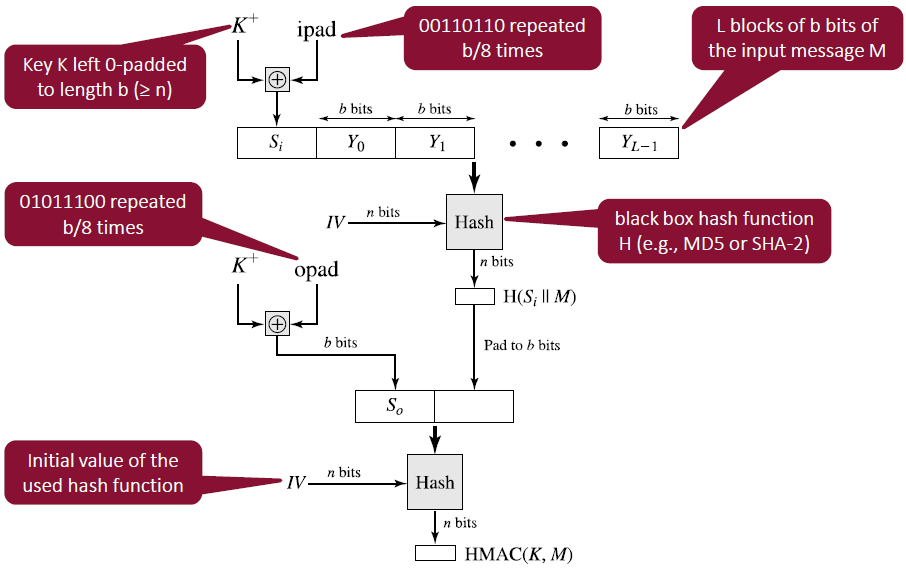
\includegraphics[width=\linewidth]{./slides/L3P5HMAC.PNG}
 	\item Cryptographic strengths:
 	\begin{itemize}
 		\item HMAC can be proven secure provided that the embedded hash function has some reasonable cryptographic strengths.
 		\item A successful attack on HMAC is equivalent to one of the following:
 		\begin{itemize}
 			\item The attacker is able to compute an output of the compression function.
 			\item The attacker finds collisions in the hash function.
 		\end{itemize}
 	\end{itemize}
 \end{itemize}

 \newpage
 \section{Asymmetric encryption}
 \subsection{Introduction}
 Asymmetric encryption uses both a public and private key, it's working is based on mathematical functions rather than substitution and permutations.\\
 AE addresses two concerns with symmetric encryption:
 \begin{itemize}
 	\item Secret keys are distributed using a trusted key distribution center
 	\item It does not enable digital signatures
 \end{itemize}
 \subsubsection{Confidentiality using AE}
 Assume there is some source A that produces a message in plaintext X which is intended for destination B. B generates a related pair of keys: a public key, $PU_b$, and a private key, $PR_b$. $PR_b$ is known only to B, whereas $PU_b$ is publicly available and therefore accessible by A.\\ With the message X and the encryption key $PU_b$ as input, A forms the ciphertext $Y = E(PU_b, X)$. The intended receiver, in possession of the matching private key, is able to invert the transformation: $X = D(PR_b,Y)$.\\ 
 An adversary, observing Y and having access to $PU_b$, but not having access to $PR_b$ or X, must attempt to recover X and/or $PR_b$. It is assumed that the adversary does have knowledge  of  the  encryption  (E)  and decryption  (D) algorithms.  If  the adversary is interested only in this particular message, then the focus of effort is to recover X by generating a plaintext estimate $\widehat{X}$. Often, however, the adversary is interested in being able to read future messages as well, in which case an attempt is made to recover $PR_b$ by generating an estimate $\widehat{PR_b}$.
 
 \subsubsection{Authentication using AE}
 In this case, A prepares a message to B and encrypts it using A’s private key before transmitting it. B can decrypt the message using A’s public key. Because the message was encrypted using A’s private key, only A could have prepared the message.Therefore,the entire encrypted message serves as a digital signature. In addition, it is impossible to alter the message without access to A’s private key, so the message is authenticated both in terms of source and in terms of data integrity.\\
 In this scheme, the entire message is encrypted, which, although validating both author and contents, requires a great deal of storage. Each document must be kept in plaintext to be used for practical purposes. A copy also must be stored in ciphertext so that the origin and contents can be verified in case of a dispute. A more efficient way of achieving the same results is to encrypt a small block of bits that is a function of the document. Such a block, called an \underline{authenticator}, must have the property that it is infeasible to change the document without changing the authenticator. If the authenticator is encrypted with the sender’s private key, it serves as a signature that verifies origin, content, and sequencing.
 
 \subsubsection{Combining confidentiality and authentication}
 It is possible to provide both the authentication function and confidentiality by a double use of the public-key scheme
 \begin{itemize}
 	\item $Z = E(PU_b,E(PR_a,X))$
 	\item $X = D(PU_a,D(PR_b,Z))$
 \end{itemize} 
 where $(PU_a, PR_a)$ is a key pair generated by the sender and is used for authentication and $(PU_b, PR_b)$ is a key pair generated by the receiver and is used for confidentiality.\\
 Encryption of a message $M$ then goes as follows: $M \rightarrow E(M, PR_a) \rightarrow E(E(M, PR_a), PU_b) \rightarrow C$.\\
 Decryption of a ciphertext $C$ happens as follows: $C \rightarrow D(C, PR_b) \rightarrow D(D(C, PR_b), PU_a) \rightarrow M$.
 
 \subsubsection{Requirements for public-key cryptography}
 \begin{itemize}
 	\begin{multicols}{2}
 		\item It is computationally easy to generate the key pair $(PU_b, PR_b)$.
 		\item It is computationally easy, given the public key $PU_b$ and a message $M$, to generate the corresponding ciphertext $C = E(PU_b, M)$.
 		\item It is computationally easy, given the private key $PR_b$ and a ciphertext $C$, to recover the plaintext $M = D(PR_b, C) = D(PR_b, E(PU_b, M))$.
 		\item It is computationally infeasible, knowing $PU_b$ or $PR_b$, to generate the other key.
 		\item It is computationally infeasible, knowing $PU_b$ and ciphertext $C$, to recover the original message $M$.
 		\item Optional: the two keys can be applied in any order.
 	\end{multicols}
 \end{itemize}
 
 \subsection{Rivest-Shamir-Adleman (RSA)}
 \subsubsection{RSA basics}
 In RSA, each plaintext block $M$ is represented by a number smaller than $n$, resulting in a block size of at most $^2log(n)+1$ bits. In practice a block size of $i$ bits is used with $2^i\leq n\leq 2^{i+1}$.\\
 Encryption and decryption happen according to following formulas:
 \begin{itemize}
 	\item Encryption: $C = M^e \text{ mod }n$
 	\item Decryption: $M = C^d \text{ mod }n = M^{ed} \text{ mod } n$
 \end{itemize}
Since both sender and receiver know $n$, only the sender knows $e$ and $d$ is known only to the receiver, the public key $PU$ en private key $PB$ become
\begin{itemize}
	\item $PU = \{e, n\}$
	\item $PB = \{d, n\}$
\end{itemize}
\textbf{Finding suitable values for $e, d$ and $n$}\\
Assuming $M$ and $n$ are relative prime, Euler's theorem states 
\begin{equation*}
M^{\phi(n)+1} \equiv M \text{ mod } n = M^{ed} \text{ mod } n \Leftrightarrow ed \equiv 1 \text{ mod }\phi(n) \Leftrightarrow d \equiv e^{-1}\text{ mod }\phi(n)
\end{equation*}
where $\phi(n)$ is the Euler totient function that returns the number of integers $k (1\leq k\leq n)$ for which $gcd(n, k) = 1$.\\
\textbf{How to guarantee $M$ and $n$ relative prime}\\
If $n = pq$ with $p$ and $q$ prime, then $M$ and $n$ are relative prime if $M$ is different from $1, p$ and $q \Rightarrow \phi(n) = (p-1)(q-1) (\Rightarrow ed\text{ mod }\phi(n) = 1)$.
 \subsubsection{RSA ingredients}
  \begin{itemize}
 	\begin{multicols}{2}
 		\item Two prime numbers $p$ and $q$, chosen privately
 		\item Integer $n = pq$, calculated and publicly available
 		\item Value $e$ chosen by key generator with $gcd(\phi(n), e) = 1; 1<e<\phi(n)$ publicly available
 		\item Value $d \equiv e^{-1}\text{ mod }\phi(n)$ calculated and private 
 	\end{multicols}
 \end{itemize}
Note that it should be infeasible to calculate $p, q$ and that this is the case if $n$ is large enough.
 
 \subsection{Efficient RSA operations}
 \subsubsection{Efficient exponentiation in modular arithmetic}
 To avoid integer overflow during calculations, we can use the property that $[(a\text{ mod }n)(b\text{ mod }n)]\text{ mod }n = (ab)\text{ mod }n$. Similarly we can make calculating large exponents more efficient by reusing intermediary results, eg $x^{13} = x*x^4*x^8$. We can calculate $x\text{ mod }n$, $x^2\text{ mod }n$, $x^4\text{ mod }n$ and $x^8\text{ mod }n$ where each reuses the previous result.\\
 $\Rightarrow$ \textbf{Algorithm to find $a^b\text{ mod }n$}\\
 $b$ can be expressed as a binary number $b_kb_{k-1}...b_1b_0$, or $b = \Sigma_{b_i\ne 0}2^i$, therefore $a^b = a^{\Sigma_{b_i\ne 0}2^i} = \Pi_{b_i\ne 0}a^{2^i}$.\\
 $\Rightarrow a^b\text{ mod }n = [\Pi_{b_i\ne 0}a^{2^i}]\text{ mod }n = [\Pi_{b_i\ne 0}a^{2^i}\text{ mod }n]\text{ mod }n $\\
 $\Rightarrow$Algorithm:
 \begin{algorithmic}
 	\State $f = 1$
 	\For {$i=k$ down to $0$}
 	\State $f = (ff)\text{ mod }n$
 	\If {$b_i = 1$}
 	\State $f = (fa)\text{ mod }n$
 	\EndIf
	\EndFor
	\State return $f$
 \end{algorithmic}
 	
 \subsubsection{Efficient operation using public key}
 To make encryption as efficient as possible, chose an exponent with few 1 bits $\rightarrow$ the most common choice is $2^{16+1}, 3, 17$ since each of these numbers only has 2 1 bits. Note that small values are vulnerable to simple attacks but that this can be solved by adding a unique psuedorandom bit string as padding.
 
 \subsubsection{Efficient operation using private key}
 If $e$ is chosen to be small, then $d$ is large by definition. To speed up calculations for large $d$ we can use the Chinese remainder theorem.\\
 We need to compute $M = C^d\text{ mod }n$. Now define $V_p = C^d\text{ mod }p$ and $V_q = C^d\text{ mod }q$. Applying the CRT gives $M = (V_pX_p + V_qX_q)\text{ mod }n$ with $X_p = q(q^{-1}\text{ mod }p)$ and $X_q = p(p^{-1}\text{ mod }q)$.\\
 Using Fermat's theorem we get that $V_p = C^{d\text{ mod }(p-1)}\text{ mod }p$ and $V_q = C^{d\text{ mod }(q-1)}\text{ mod }q$ where both $d\text{ mod }(p-1)$ and $d\text{ mod }(q-1)$ can be pre-calculated since $p, q$ and $d$ are known in advance.\\
 By doing this precalculation, calculation of $M$ is about 4 times more efficient.
 
 \subsubsection{Efficient key generation}
 \begin{enumerate}
 	\item Determine 2 prime numbers $p$ and $q$.\\
 	Any adversary will know $n=pq$, so in order to prevent brute force attacks $p$ and $q$ should be large enough and the method to find large $p$ and $q$ should be efficient.\\
 	$\rightarrow$ Generate a random uneven number with the desired order of magnitude. If the number is determined to be prime, then return it. Else we generate a new number and repeat the process.
 	\item Select $e$ or $d$ and calculate the other.\\
 	If $p$ and $q$ are found, than $n$ is found and $\phi(n) = (p-1)(q-1)$ is found. Now lets select $e$ such that $gcd(\phi(n), e) = 1$ and calculate $d$ such that $d\equiv e^{-1}(\text{ mod }\phi(n))$. Both values can be calculated simultaneously using the Extended Euclids Algorithm. \\
 	One possible strategy is to select random numbers $e$ until one is relative prime to $\phi(n)$.
 \end{enumerate}
 
 \subsection{Attacks against RSA}
 \subsubsection{Brute force attacks}
 Try all possible private keys $(d, n)$. RSA is safe if $n$ is chosen large enough: minimum 3072 bits for $n$ with RSA, in symmetric encryption 128 suffice.
 
 \subsubsection{Mathematical attacks}
 Factor the product of $p$ and $q$ given $n$. There are 3 approaches to this kind of attack.
 \begin{enumerate}
 	\item Factor $n$ into 2 primes $p$ and $q$
 	\item Determine $\phi(n)$ directly without finding $p$ and $q$
 	\item Determine $d$ directly without finding $\phi(n)$
 \end{enumerate}
The first two options are mathematically equivalent and easier than the last option.\\
This gives rise to 2 threats to the use of large key sizes:
\begin{itemize}
	\item Continuously improving computational power
	\item Refinement of factoring algorithms
\end{itemize}
There are a few safety precautions that can be taken:
\begin{itemize}
	\item $p$ and $q$ should be nearly the same number of digits
	\item Both $(p-1)$ and $(q-1)$ should contain a large prime factor
	\item $gcd(p-1, q-1)$ should be small
\end{itemize}

 \subsubsection{Timing attacks}
 Exploit the running time of decryption algorithm. This is a ciphertext only attack where a snooper can determine the private key by keeping track of how long it takes to decipher the message. It is applicable to all public key encryption algorithms and for RSA, it uses the timings of the modular exponentiation algorithm. Counter measures include constant exponentiation time (which leads to degraded performance), adding a random delay or by using the blinding technique.\\
 In the blinding technique the operation $M=C^d\text{ mod }n$ is replaced by
 \begin{enumerate}
 	\item Generate a random number $r \in ]0, n-1]$
 	\item Compute $C' =Cr^e \text{ mod }n$ where $e$ is the public exponent
 	\item Compute $M' = (C')^d \text{ mod } n$
 	\item Compute $M = M'r^{-1}$ 
 \end{enumerate}
 This method results in a 2-10\% performance loss.
 
 \subsubsection{Chosen ciphertext attacks}
 Exploit properties of RSA. In this attack the attacker chooses some ciphertext and is given the corresponding plaintext in return. Another possibility is that the attacker sends chosen blocks of data that yield additional information useful for cryptoanalysis.\\
 Given the property that $E(PU,M_1)xE(PU,M_2) = E(PU, M_1xM_2)$ and $C=M^e\text{ mod }n$, we can derive $M$ using the CCA attack as follows
 \begin{itemize}
 	\item Compute $x = (Cx2^e)\text{ mod }n$
 	\item Submit $x$ as a chosen ciphertext and receive $y = x^d\text{ mod }n$
 \end{itemize}
$\Rightarrow x = (C\text{ mod }n)x(2^e\text{ mod }n) = (M^e\text{ mod }n)x(2^e\text{ mod }n) = (2M)^e\text{ mod }n$\\
Therefore $y = (2M)\text{ mod }n$, from which $M$ can be easily deduced.
 
 \subsection{Digital signatures}
 \subsubsection{Introduction}
 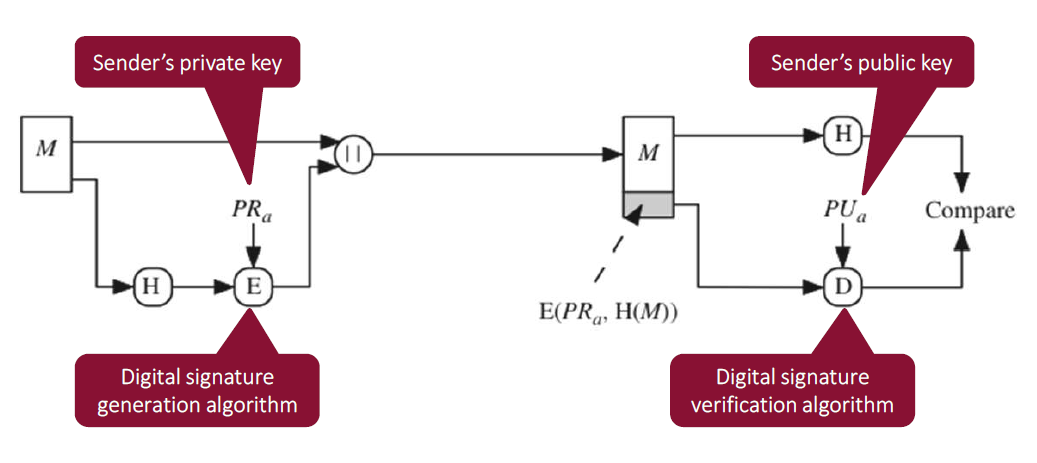
\includegraphics[width=\linewidth]{./slides/L4P5intro.PNG}\\
 Authentication vs signatures:
 \begin{itemize}
 	\item Authentication: protects against third parties, only use single private key which is securely shared between sender and receiver $\rightarrow$ verify content of message was not altered.
 	\item Signatures: provides additional securities, ensures that anyone can verify that the message was indeed sent by the sender.
 \end{itemize}
 \subsubsection{Required properties of a digital signature}
 A digital signature must:
 \begin{enumerate}
 	\item Verify the author and time of the signature $\rightarrow$ avoid misuse of private key
 	\item Authenticate the contents at the time of the signature
 	\item Be verifiable by third parties to resolve disputes $\rightarrow$ cannot be provided by MAC
 \end{enumerate}
 
 \subsubsection{RSA-PSS}
 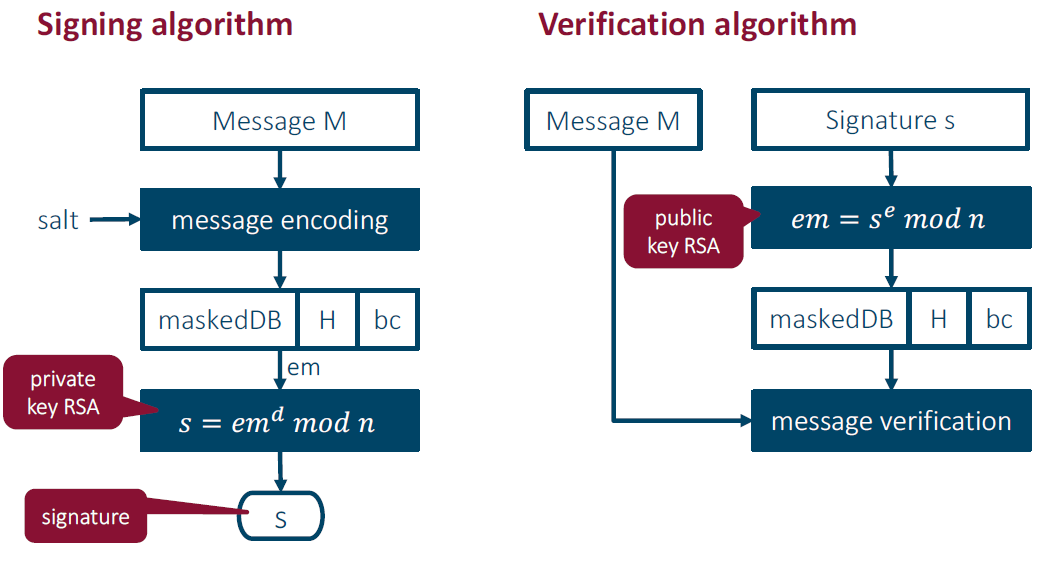
\includegraphics[width=\linewidth]{./slides/L4P5RSAPSS.PNG}\\
 We discuss the RSA Probabilistic Signature Scheme (RSA-PSS), which is the latest of  the RSA schemes and the one that RSA Laboratories recommends as the most secure of the RSA schemes.\\
 We show how the signature is formed by a signer with private key $\{d, n\}$ and public key $\{e, n\}$. Treat the octet string $EM$ as an unsigned, nonnegative binary integer $m$. The signature $s$ is formed by encrypting $m$ as follows: $s = m^d \text{mod} n$.\\
 Let $k$ be the length in octets of the RSA modulus $n$. For example if the key size for RSA is 2048 bits, then $k$ = 2048/8 = 256. Then convert the signature value $s$ into the octet string $S$ of length $k$ octets.\\
 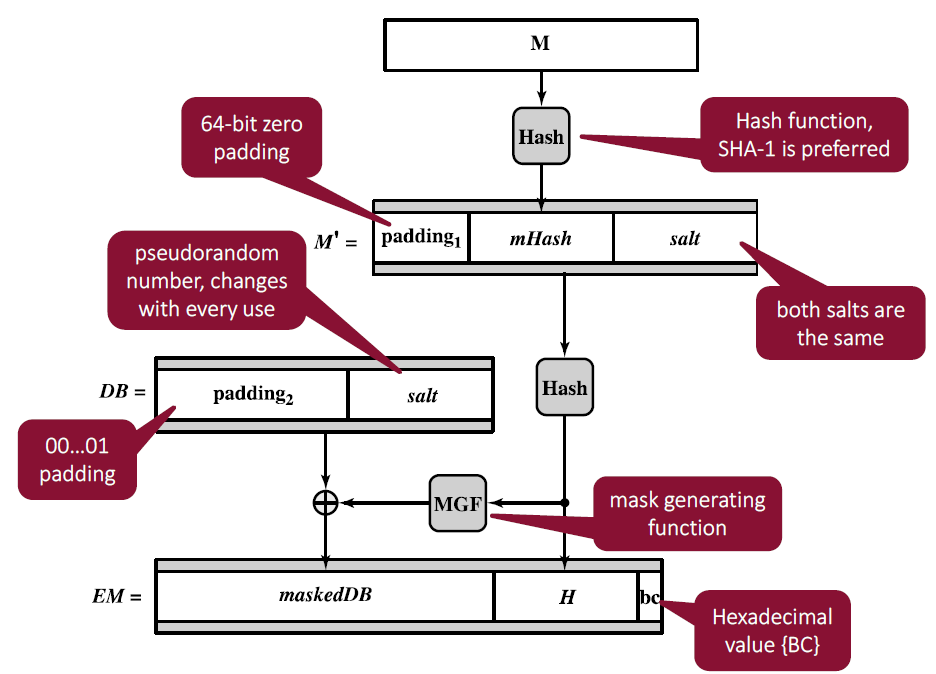
\includegraphics[width=\linewidth]{./slides/L4P5RSAPSSENC.png}\\
 The first stage in generating an RSA-PSS signature of a message $M$ is to generate from $M$ a fixed-length message digest, called an encoded message. We define the following parameters and functions:
 \begin{itemize}
 	\item  Options
 	\begin{itemize}
 		\item Hash: hash function with output hLen octets. The current preferred alternative is SHA-1, which produces a 20-octet hash value.
 		\item MGF: mask generation function. The current specification calls for MGF1.
 		\item $sLen$: length in octets of the salt. Typically sLen = hLen, which for the
 		current version is 20 octets.
 	\end{itemize}
 	\item Input
 	\begin{itemize}
 		\item $M$: message to be encoded for signing.
 		\item $emBits$: This value is one less than the length in bits of the RSA modulus n.
 	\end{itemize}
 	\item Output
 	\begin{itemize}
 		\item EM: encoded message. This is the message digest that will be encrypted to form the digital signature.
 	\end{itemize}
 	\item Parameters
 	\begin{itemize}
 		\item $emLen$: length of EM in octets = $emBits/8$.
 		\item padding1: hexadecimal string 00 00 00 00 00 00 00 00; that is, a string of 64 zero bits.
 		\item padding2 : hexadecimal string of 00 octets with a length (emLen - sLen - hLen - 2) octets, followed by the hexadecimal octet with 63 (emLen - sLen - hLen - 2) octets, followed by the hexadecimal octet with value 01.
 		\item salt: a pseudorandom number.
 		\item bc: the hexadecimal value BC.
 	\end{itemize}
 \end{itemize}
The encoding process consists of the following steps.
\begin{itemize}
	\item Generate the hash value of M: $mHash = Hash(M)$
	\item Generate a pseudorandom octet string salt and form block $M' = padding1 || mHash || salt$
	\item Generate the hash value of M': $H = Hash(M')$
	\item Form data block $DB = padding2 || salt$
	\item Calculate the $MGF$ value of H: $dbMask = MGF(H, emLen - hLen - 1)$
	\item Calculate $maskedDB = DB \bigoplus dbMsk$
	\item Set the leftmost 8 $emLen - emBits$ bits of the leftmost octet in $maskedDB$ to 0
	\item $EM = maskedDB || H || 0xbc$
\end{itemize}

 \subsubsection{RSA-PSS MGF (Mask Generating Function)}
 The goal is to generate a cryptographically secure variable length $L$ hash code using a fixed length output cryptographic hash function $H$, eg SHA.\\
 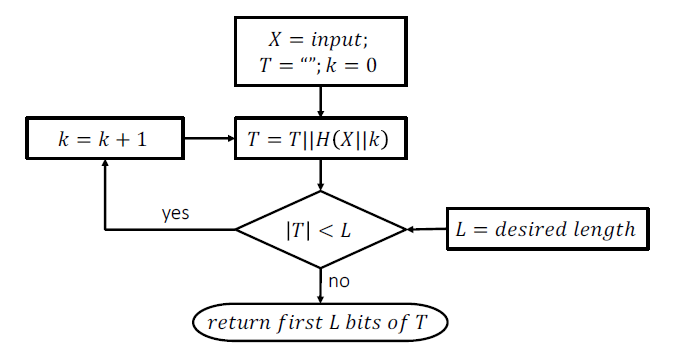
\includegraphics[width=0.8\linewidth]{./slides/L4P5RSAPSSMGF.PNG}
 
 \subsubsection{RSA-PSS signature verification}
  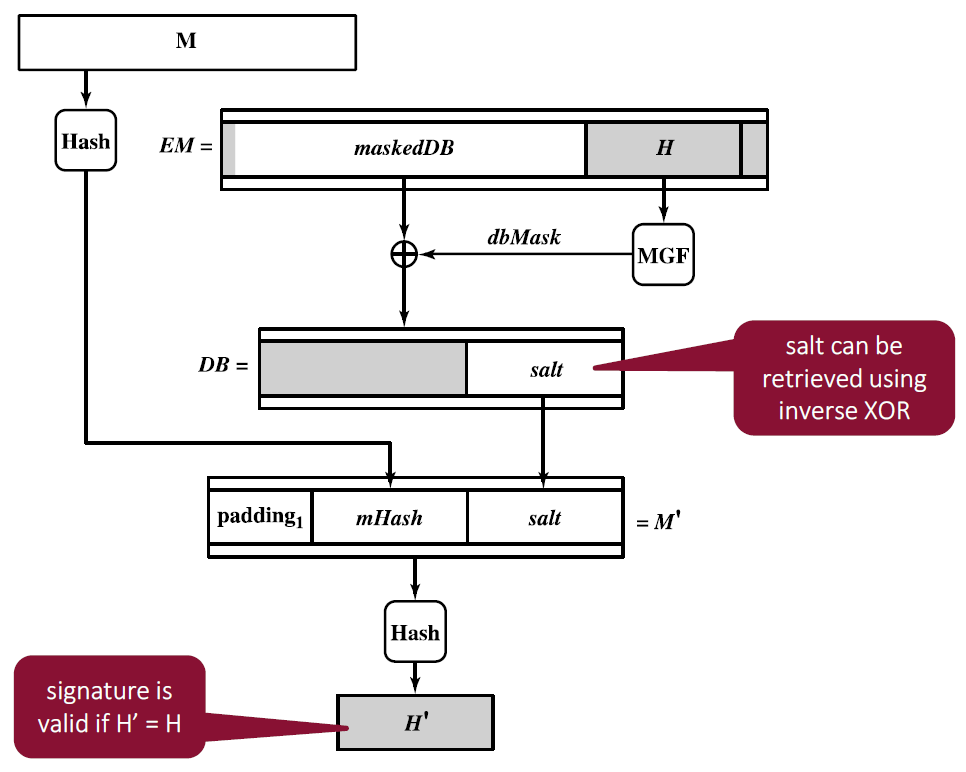
\includegraphics[width=0.8\linewidth]{./slides/L4P5RSAPSSSIGVER.PNG}\\
  For signature verification, treat the signature $S$ as an unsigned, nonnegative binary integer $s$. The message digest $m$ is recovered by decrypting $s$ as follows: $m = se \text{ mod } n$.\\
  Then, convert the message representative $m$ to an encoded message $EM$ of length $emLen = modBits -\frac{1}{8}$ octets, where $modBits$ is the length in bits of the RSA modulus $n$.

 \newpage
 \section{Key distribution}
 \subsection{Symmetric private key distribution}
 \noindent\fbox{%
 	\parbox{\textwidth}{%
 		How to share a private key between 2 parties without others having access to it?
 	}%
 }

 There are a few different distribution methods for parties $A$ and $B$:
 \begin{enumerate}
 	\item $A$ selects the key and physically delivers it to $B$
 	\item Third party selects a key and physically delivers it to $A$ and $B$
 	\item If $A$ and $B$ already share a key, a new key can be encrypted using the old key and transmitted over the network
 	\item If $A$ and $B$ have anencrypted connection to a third party $C$, $C$ can deliver a key on the encrypted link to $A$ and $B$
 \end{enumerate}
 Solutions 1 and 2 are infeasible in large scale networks. If in solution 3 an attacker determines a single key then all future keys are compromised, due to the amount of keys that need to be maintained this solution too can only be used on small scale.\\
 It thus follows that solution 4 is the preferred one.

 \subsubsection{Decentralized key control without third party}
 This way of working avoids the need for a central trusted authority, but it can only be used in small scale scenarios like local networks.\\
 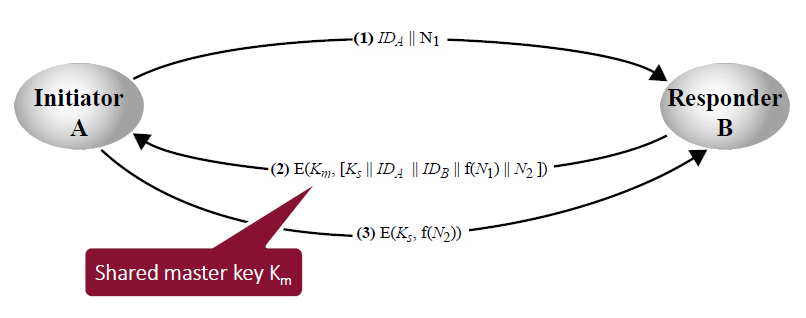
\includegraphics[width=\linewidth]{./slides/L5P1.PNG}
 \begin{enumerate}
 	\item $A$ send $ID_A||N_1$ to $B$ where $N_1$ is a random nonce
 	\item $B$ uses the previously shared master key $K_m$ to encrypt a newly generated key $K_s$
 	\item After decryption $A$ will send $E(K_s, f(N_2))$ to $B$
 \end{enumerate}
This approach uses $\frac{N(N-1)}{2}$ keys in a network with $N$ hosts.
 
 \subsection{Key Distribution Centers (KDCs)}
 \noindent\fbox{%
 	\parbox{\textwidth}{%
 		Centralized authority that distributes keys using symmetric encryption.
 	}%
 }

 \subsubsection{Hierarchical structure}
 Keys are stored on 2 levels:
 \begin{itemize}
 	\item Session keys: temporary keys used between two end systems, discarded after logical session ends.
 	\item Master keys: used to safely encrypt and transmit session keys $\rightarrow$ maintained between KDC and hosts, only used when host requests new session key.
 \end{itemize}

 \subsubsection{KDC scenario}
 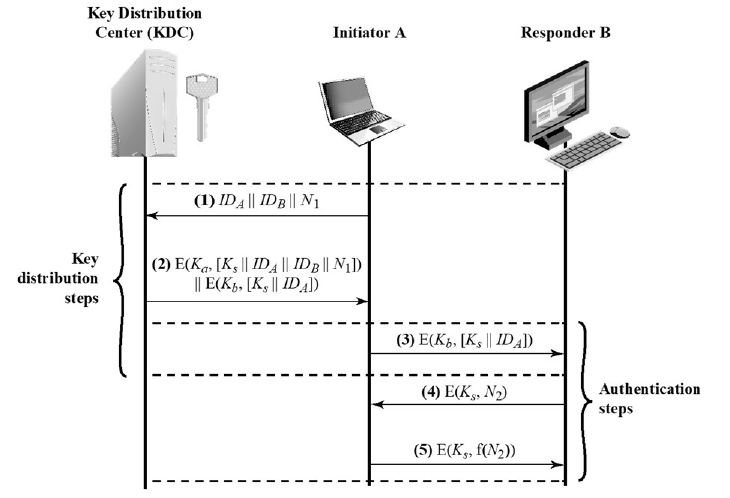
\includegraphics[width=\linewidth]{./slides/L5P2KDC.PNG}
 
 \subsubsection{Hierarchical key control}
 A hierarchy of KDCs manages different parts of an internetwork where each local KDC distributes keys in the local network.\\
 Higher layer KDCs can coordinate key distribution across networks.
 
 \subsubsection{Transparent key control scheme}
 For providing end-to-end encryption in connection-oriented protocols.
 \begin{enumerate}
 	\item Host sends packet to request connection
 	\item Security service buffers packet; asks KDC for session key
 	\item KDC distributes session key to both hosts
 	\item Buffered packet is transmitted
 \end{enumerate}
 
 \subsection{Asymmetric private key distribution}
 \subsubsection{Symmetric key distribution using asymmetric encryption}
 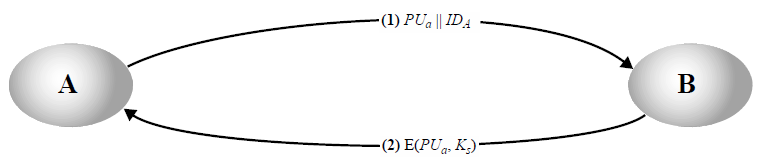
\includegraphics[width=\linewidth]{./slides/L5P3SYM.PNG}\\
 This scheme is vulnerable to "man-in-the-middle" attacks $\rightarrow$ same scheme but with an attacker in the middle\footnote{Duh}.
 
 \subsubsection{Diffie-Hellman key exchange}
 Enables 2 users to securely exchange a key (eg for use in subsequent symmetric encryption).\\
 It is based on the difficulty to calculate discrete logarithms. The exponent $i$ is the discrete logarithm of $b$ for base $a$ mod $p$: $d\text{ log}_{a,p}(b)=i \Leftrightarrow b\equiv a^i\text{ mod }p$.\\
 Parties share the publicly known pair $(q,\alpha)$ where $q$ is a prime number and $\alpha$ is an integer and prime root of $q$, meaning a unique exponent $i$ exists for every integer $b<q$ such that $b\equiv\alpha^i\text{ mod }q$.\\
 Private keys are random number $X_A$ and $X_B$ both smaller than $q$. The public keys are $Y_A = \alpha^{X_A}\text{ mod }q$ and $Y_B = \alpha^{X_B}\text{ mod }q$. The shared secret key $K = (Y_B)^{X_A}\text{ mod }q = (Y_A)^{X_B}\text{ mod }q$ can be calculated.\\
 To an attacker, $q, \alpha, Y_A$ and $Y_B$ are available. This means that the private key of $B$ can be calculated as $X_B=d\text{ log}_{\alpha, q}(Y_B)$. The security of Diffie-Hellman lies in the fact that it is easy to calculate exponentials modulo a prime number but that it is hard to calculate discrete logarithms.\\
 The "man-in-the-middle" attack is still possible.
 
 \subsection{Secure distribution of public keys}
 There are 4 general techniques for public key distribution:
 \begin{enumerate}
 	\item Public announcement: broadcast public keys to anyone
 	\item Public directory: dynamic centralized directory of keys
 	\item Public key authority: tightly controlled central directory
 	\item Public key certificates: decentralized secure key exchange
 \end{enumerate}
Both (1) and (2) are not safe, (3) has scalability issues due to the central nature. Hence, (4) is the preferred solution due to better scalability.
 
 \subsubsection{Public announcement}
 Since there is no form of control, anyone can forge an announcement and pretend to be $A$, spreading their own public key.
 
 \subsubsection{Public directory}
 Keys are registered in person or using secure authenticated communication. If the directory's private key is stolen, an attacker can counterfeit public keys.
 
 \subsubsection{Public key authority}
 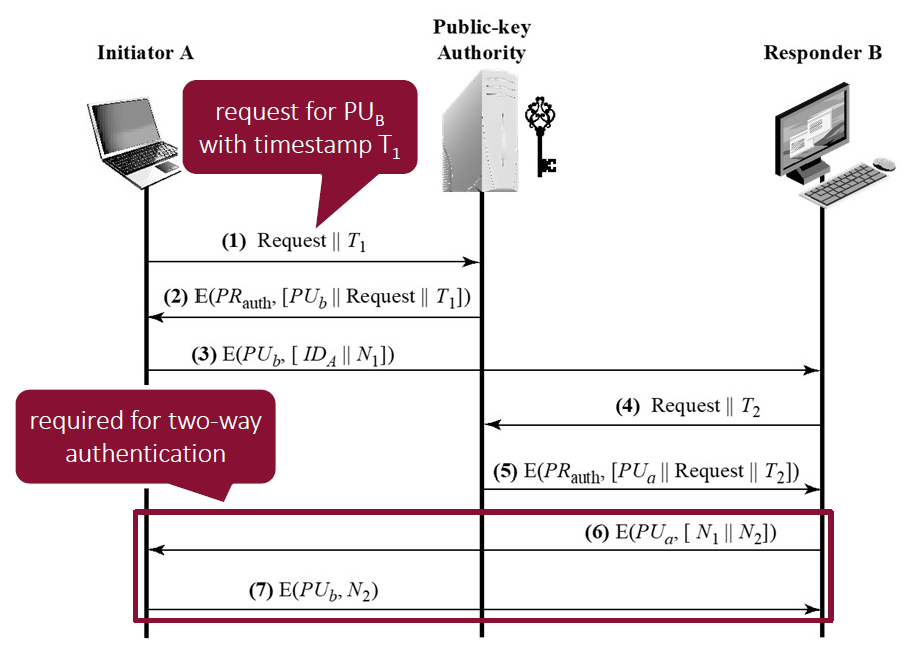
\includegraphics[width=\linewidth]{./slides/L5P4PKA.PNG}
 
 \subsubsection{Certificates} 
 Central authority only used to generate a certificate that consists of the public key, the ID of the owner the trusted third party's signature. A certificate must adhere to following requirements:
 \begin{itemize}
 	\item Any participant can determine the name and public key of the owner
 	\item Any participant can verify that the certificate originated from the certificate authority and is not counterfeit
 	\item Only the certificate authority can create and update certificates
 	\item Any participant can verify the time validity of the certificate
 \end{itemize}
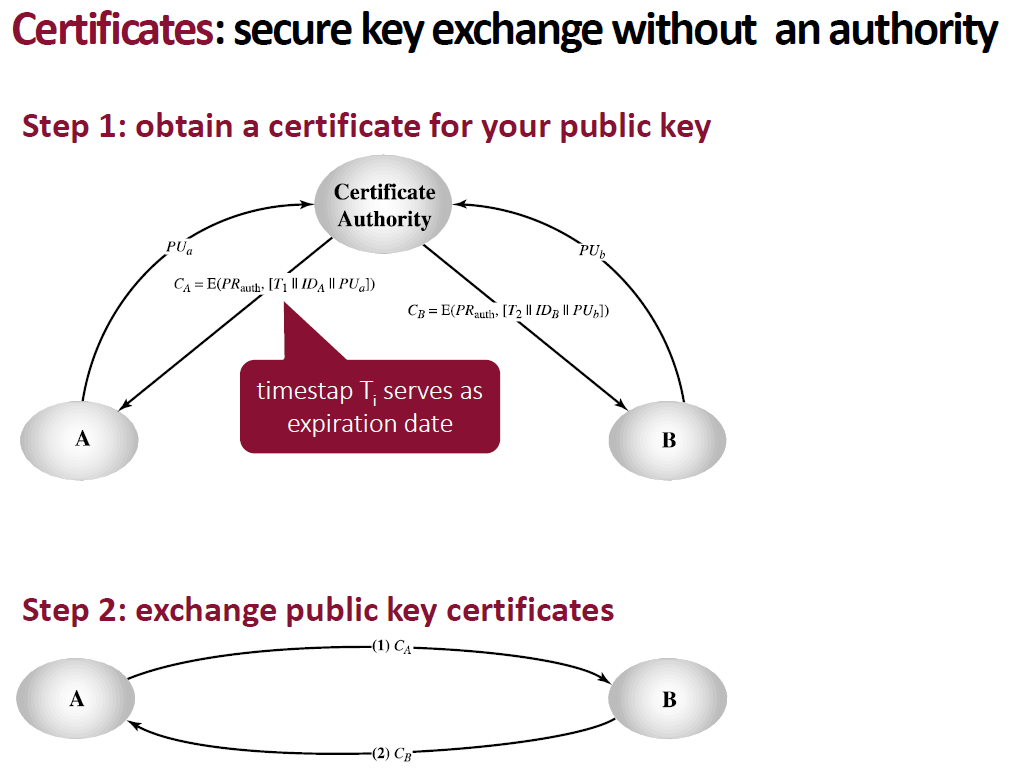
\includegraphics[width=0.8\linewidth]{./slides/L5P4CERT.PNG}
 
 \subsection{X.509 certificates}
 
 \subsubsection{Certificate generation/working}
 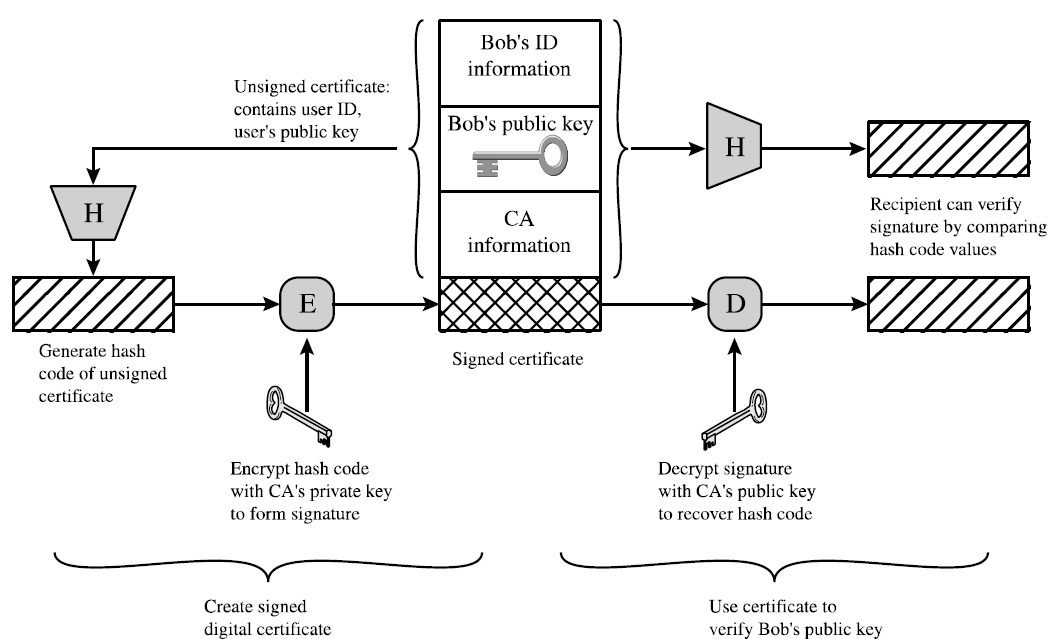
\includegraphics[width=\linewidth]{./slides/L5P5WORK.PNG}
 
 \subsubsection{X.509 format}
 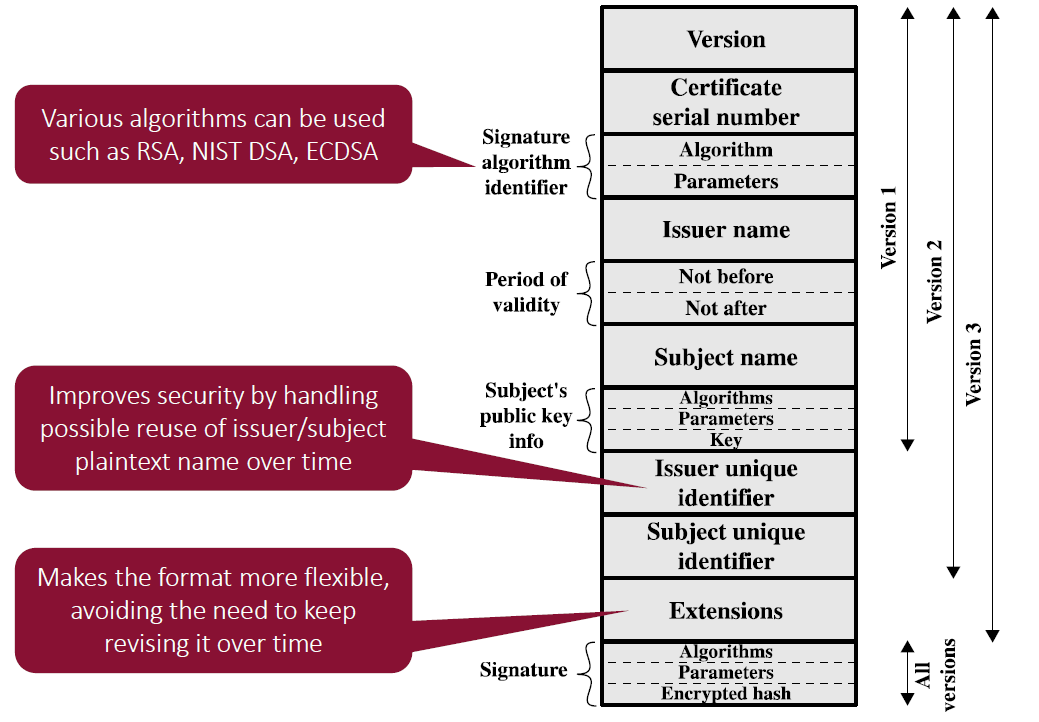
\includegraphics[width=\linewidth]{./slides/L5P5FORM.PNG}
 
 \subsubsection{CA organization}
 
 If the user community is large, eg the internet, then multiple CA's are needed.\\
 \noindent\fbox{%
 	\parbox{\textwidth}{%
 		$Y<<X>>$: certificate of user $X$ is issued by CA $Y$.
 	}%
 }
 \begin{figure}[H]
 	\begin{subfigure}{.7\textwidth}
 		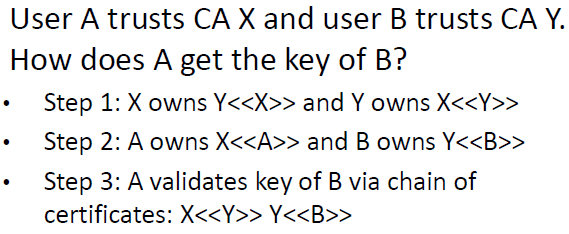
\includegraphics[width=.8\linewidth]{./slides/L5P5ORG1.PNG}
 	\end{subfigure}%
 	\begin{subfigure}{.7\textwidth}
 		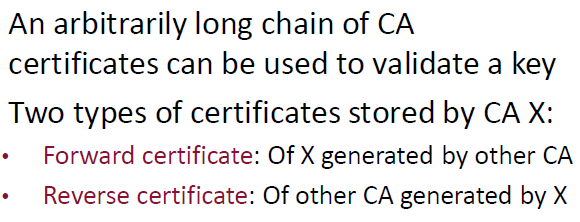
\includegraphics[width=.8\linewidth]{./slides/L5P5ORG2.PNG}
 	\end{subfigure}
 \end{figure}
 
 \subsubsection{Certificate revocation}
 
\begin{multicols}{2}
	Revocation may be needed if:
	\begin{itemize}
		\item User's private key is possibly compromised
		\item User is no longer certified by CA
		\item CA's certificate is possibly compromised
	\end{itemize}
	Each CA maintains a CRL (certificate revocation list) with all non-expired but revoked certificates. \\
	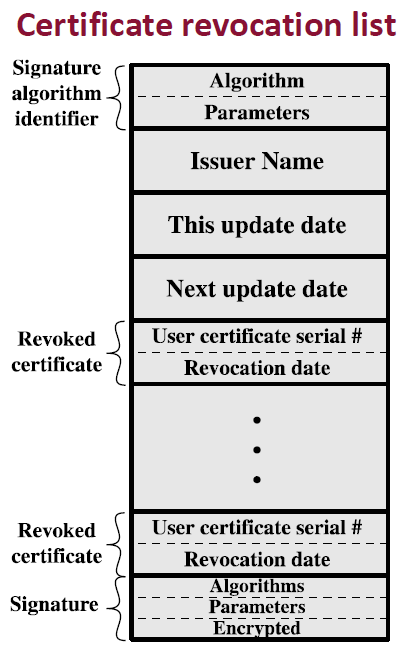
\includegraphics[width=\linewidth]{./slides/L5P5CRL.PNG}
\end{multicols}

 
 \subsubsection{Certificate extensions field}
 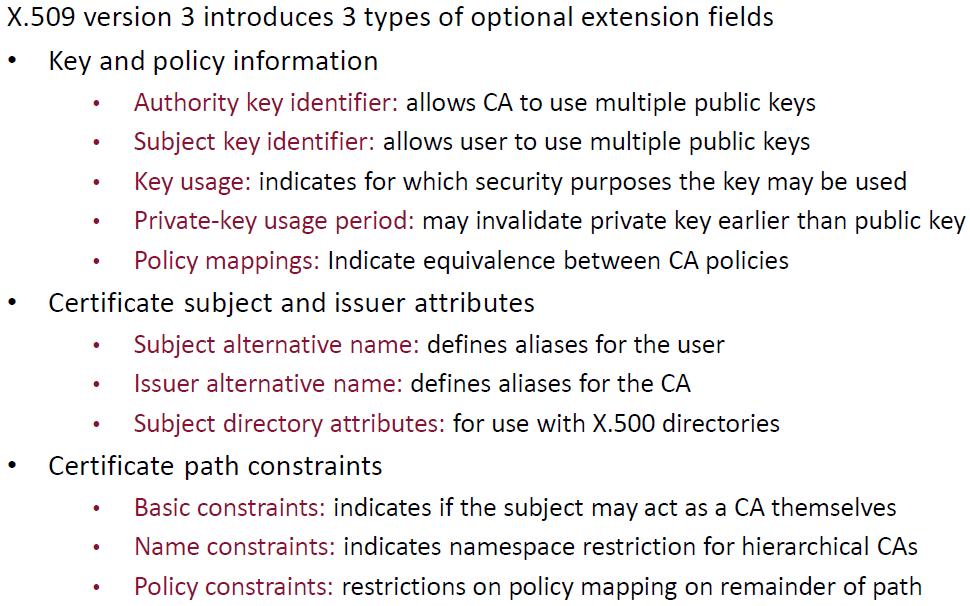
\includegraphics[width=\linewidth]{./slides/L5P5EXT.PNG}
 
 \subsubsection{Public Key Infrastructure (PKI)}
 Set of hardware, software, people, policies and procedures needed to create, manage, store, distribute and revoke digital certificates based on asymmetric cryptography.\\
 PKI objective: enable secure, convenient and efficient acquisition of public keys.\\
 $\rightarrow$ PKI X.509: formal, generic model based on X.509 to deploy certificate-based architecture on the internet.\\
 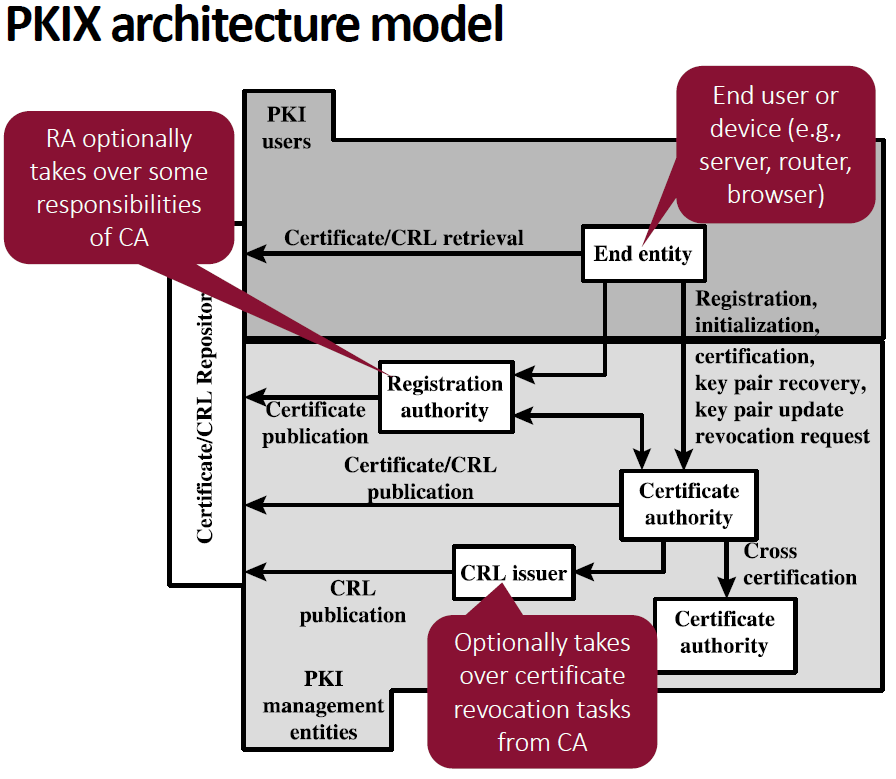
\includegraphics[width=\linewidth]{./slides/L5P5PKIMOD.PNG}\\
 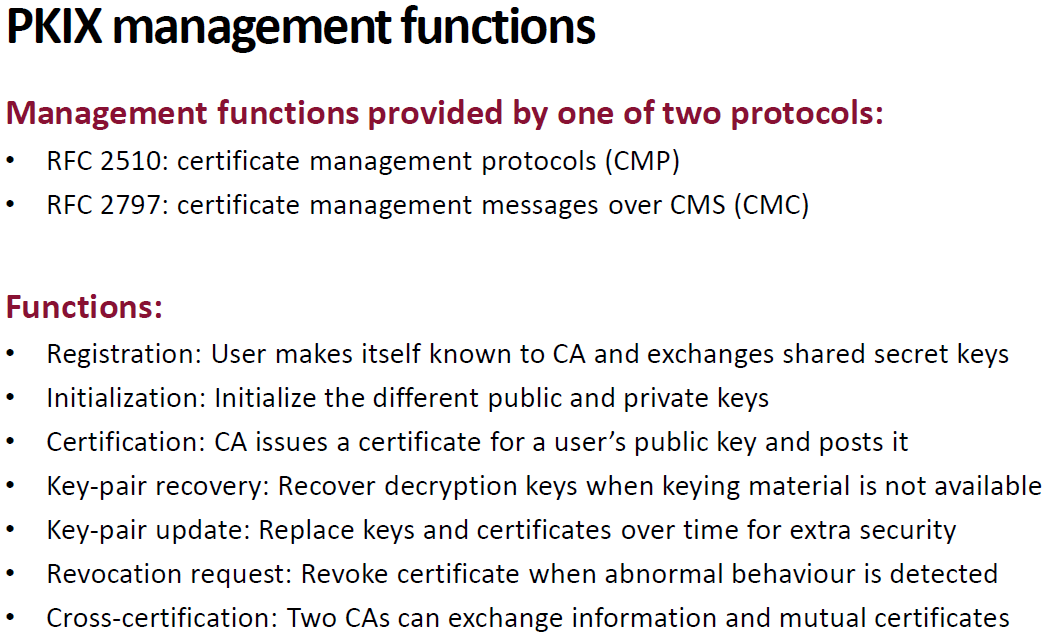
\includegraphics[width=\linewidth]{./slides/L5P5PKIMAN.PNG}
 
 \newpage
 \section{Access Control}
 \subsection{Authentication and authorization}
 Access control refers to the combination of both authentication and authorization. \\
 \noindent\fbox{%
 	\parbox{\textwidth}{%
 		Authentication: verify identity of a system entity (eg user).\\
 		Authorization: verify entity's right to perform specific actions.
 	}%
 }
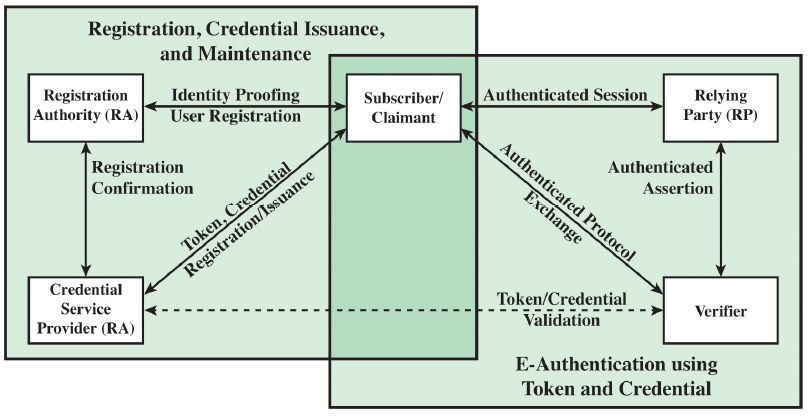
\includegraphics[width=\linewidth]{./slides/L6P1AUTHMOD.PNG}\\
The above scheme depicts how authentication happens:
\begin{itemize}
	\item In a first step, a subscriber will proof its identity to the Registration Authority (RA). The RA will then interface with the Credential Service Provider (CSP) to confirm the registration and CSP will provide the user with a token or credentials.
	\item In the second step, the user contacts a verifier via an authenticated protocol exchange. This verifier will then verify the credentials with the CSP and if this proves successful the verifier will relay to relying party to authenticate the user.
\end{itemize}
The means of authentication include  what the user:
\begin{itemize}
	\item knows: password, pin, questions, ...
	\item has: key, token generator, ...
	\item is: fingerprint, iris, ...
\end{itemize}
Multifactor authentication combines multiple methods to improve security.\\
\textbf{\underline{Access control:}}
\begin{multicols}{2}
	\begin{itemize}
		\item Functions
		\begin{itemize}
			\item Authenticates users login into the system
			\item Determines what data logged in users can access
			\item Determines what actions logged in users can perform
			\item Examines the health of the user's device
		\end{itemize}
		\item Enforcement methods
		\begin{itemize}
			\item IEEE802.1x
			\item Firewalls
			\item VLANs
			\item DHOP management
		\end{itemize}
		\item Related technologies and support systems
		\begin{itemize}
			\item Intrusion detection
			\item IPSecurity
		\end{itemize}
	\end{itemize}
\end{multicols}

 
 \subsection{Network Access Control (NAC)}
 \subsubsection{Network access control}
 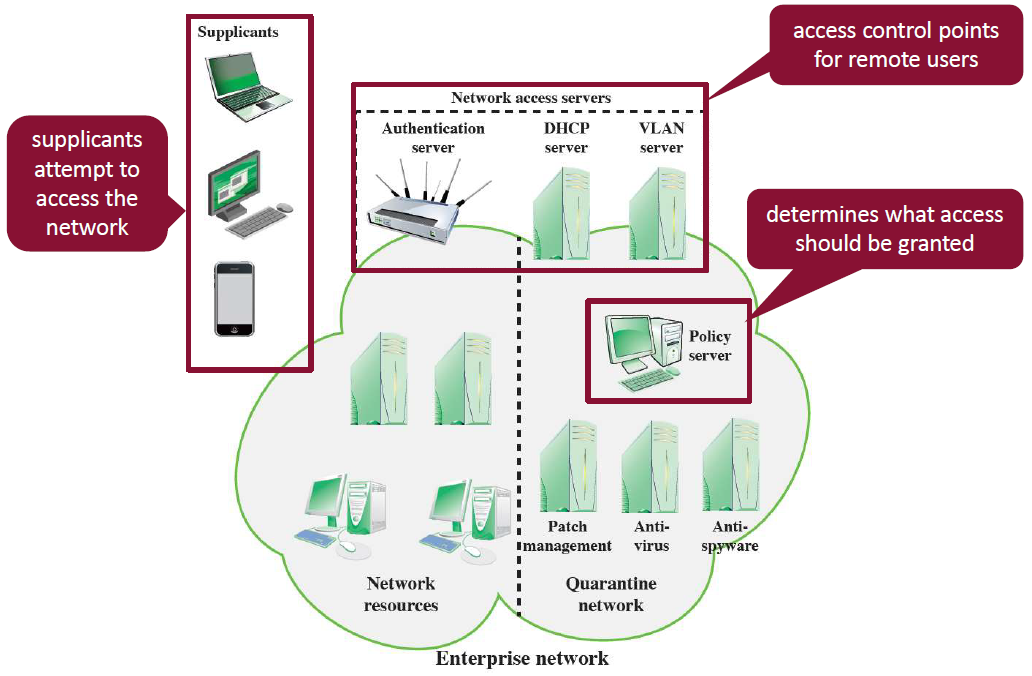
\includegraphics[width=\linewidth]{./slides/L6P2NAC.PNG}\\
 As we can see there are 3 actors:
 \begin{itemize}
 	\item Supplicants: attempts to access the network, can be any IP based device
 	\item Policy server: determines what access should be granted to supplicant, relies in back end services such as patch management, anti-virus, anti-spyware, user directory
 	\item Network access server: access control points for remote users, can be an authentication server or DHCP/VLAN server
 \end{itemize}
 
 \subsubsection{Extensible authentication protocol (EAP)}
 Provides a set of protocol messages that can encapsulate various authentication methods to be used between a supplicant and an authentication server. As such, it enables authentication over a network between hosts in the network. It can also operate over a variety of link layer facilities and technologies such as point-to-point links, LAN, WIFI, ...\\
 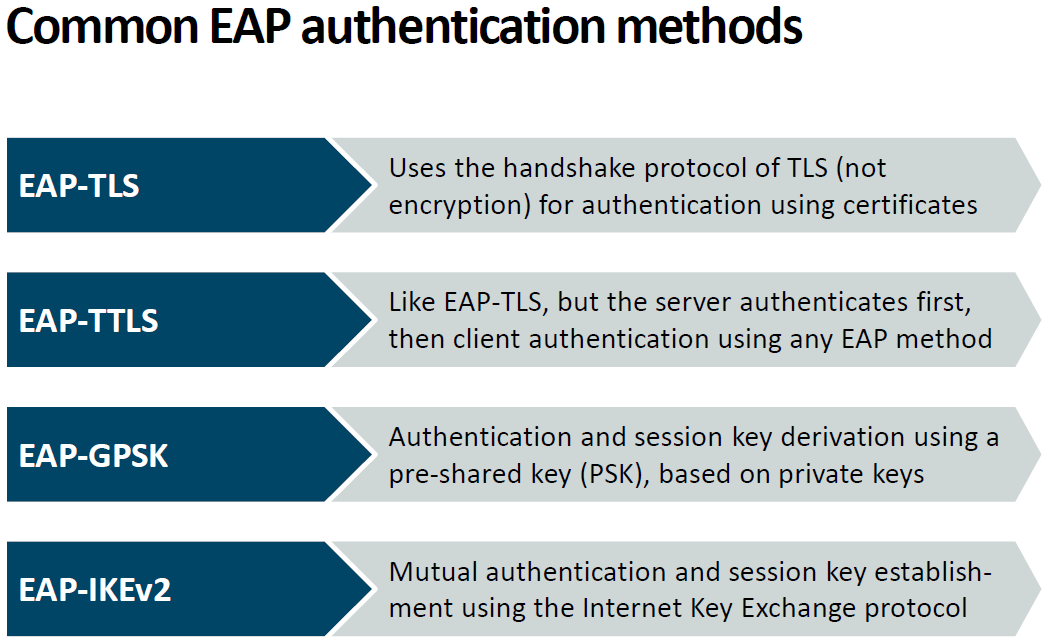
\includegraphics[width=\linewidth]{./slides/L6P2EAPAUTH.PNG}\footnote{IMPORTANT}\\  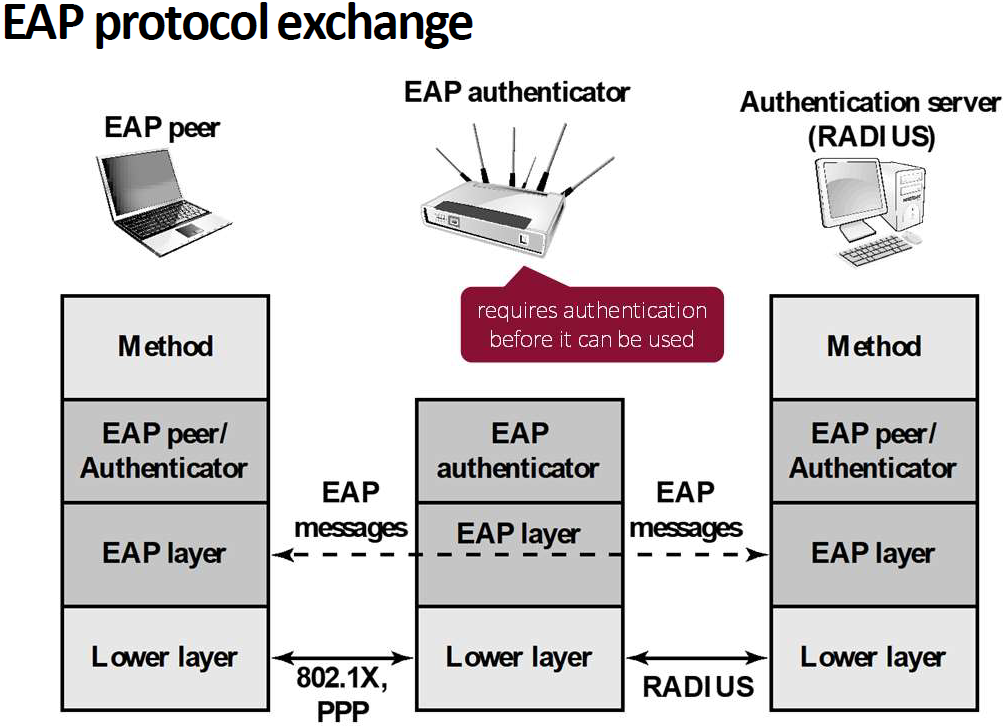
\includegraphics[width=0.8\linewidth]{./slides/L6P2EAPEXCH.PNG}
 
 \subsubsection{802.1x port based NAC}
 Enables access control in LANs, such as ethernet and wifi, and is based on a concept of port-based network access control. This means that it was a concept of controlled and uncontrolled ports. These ports are logical entities defined by the authenticator and refer to physical network connections.\\
 An uncontrolled port allows exchange of data between the supplicant and the authentication server regardless of the authenticated state. This means that control messages and messages of authentication exchange such as EAP protocol messages are always allowed into the network by th network access point, but only once the authenticator has authenticated the supplicant the controlled ports are opened allowing the exchange of actual data traffic between the external supplicant and internal network.
 
 \subsubsection{802.1x EAP over LAN (EAPOL)}
 Enables the message exchange between a supplicant, an authenticator and authentication server.\\
 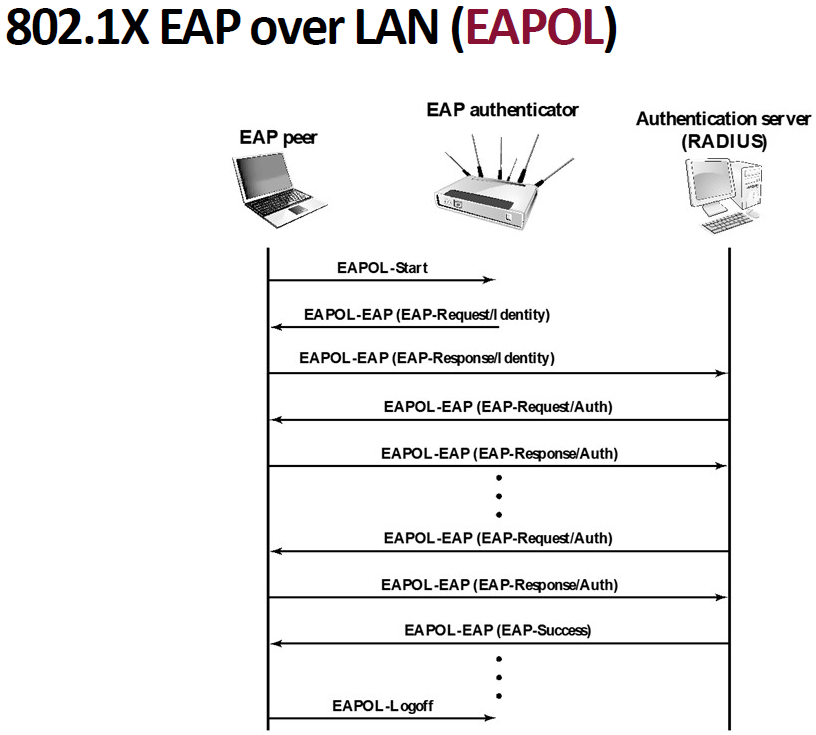
\includegraphics[width=\linewidth]{./slides/L6P2EAPOL.PNG}
 
 \subsection{Firewalls}
 Design goals:
 \begin{enumerate}
 	\item All traffic in and out must pass through the firewall
 	\item Only authorized traffic is allowed to pass through
 	\item The firewall is immune to penetration
 \end{enumerate}
Firewalls can use traffic filtering properties to determine whether to allow traffic or not (eg source and dest IP, port numbers, protocols, ...).
 
 \subsubsection{Firewall types}
 In increasing order of effectiveness:
 \begin{enumerate}
 	\item Packet filtering type: network access rules are applied to each packet separately, which is then forwarded or discarded. The packet filter is typically set up as a list of rules based on matches to fields in the IP or TCP header. If there is a match to one of the rules, that rule is invoked to determine whether to forward or discard the packet. If there is no match to any rule, then a	default action is taken. Two default policies are possible:
 	\begin{itemize}
 		\item Default = discard: That which is not expressly permitted is prohibited (whitelisting).
 		\item Default = forward: That which is not expressly prohibited is permitted (blacklisting).
 	\end{itemize}
 	The default discard policy is more conservative. Initially, everything is blocked, and services must be added on a case-by-case basis. This policy is more visible to users, who are more likely to see the firewall as a hindrance. However, this is the policy likely to be preferred by businesses and government organizations. Further, visibility to users diminishes as rules are created. The default forward policy increases ease of use for	end users but provides reduced security; the security administrator must, in essence, react to each new security threat as it becomes known. This policy may be used by	generally more open organizations, such as universities. This kind of filtering works on the transport layer.\\
 	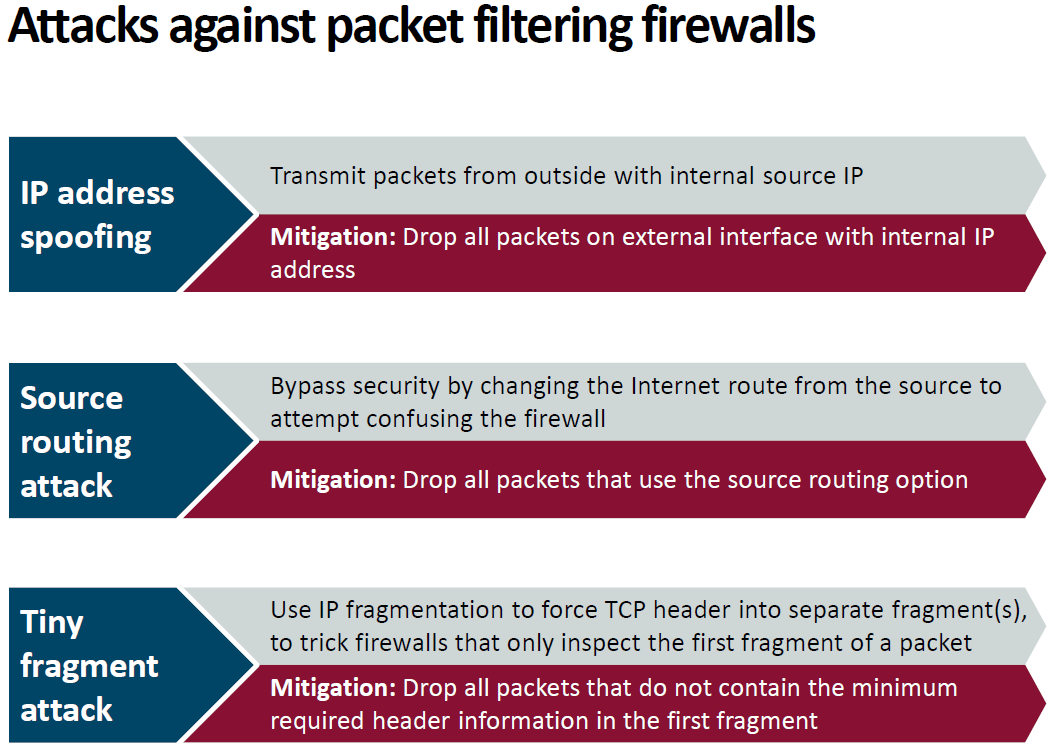
\includegraphics[width=\linewidth]{./slides/L6P3F1ATT.PNG}
 	\item Stateful inspection: keeps track of outbound TCP connections, so only currently active TCP ports have to be opened.\\
 	A stateful packet inspection firewall reviews the same packet information as a packet filtering firewall, but also records information about TCP connections. Some stateful firewalls also keep track of TCP sequence numbers to prevent attacks that depend on the sequence number, such as session hijacking. Some even inspect limited amounts of application data for some well-known protocols like FTP, IM and SIPS commands, in order to identify and track related connections.
 	\item Application proxy: acts as a termination point for TCP connections, relaying traffic after user authentication.\\
 	Application-level gateways tend to be more secure than packet filters. Rather than trying to deal with the numerous possible combinations that are to be allowed and forbidden at the TCP and IP level, the application-level gateway need only scrutinize a few allowable applications. In addition, it is easy to log and audit all incoming traffic at the application level.\\
 	A prime disadvantage of this type of gateway is the additional processing overhead on each connection. In effect, there are two spliced connections between the end users, with the gateway at the splice point, and the gateway must examine and forward all traffic in both directions.
 	\item Circuit-level proxy: similar to (3), but doesn't examine content after connection establishment.\\
 	As with an application gateway, a circuit-level gateway does not permit an end-to-end TCP connection; rather, the gateway sets up two TCP connections, one between itself and a TCP user on an inner host and one between itself and a TCP user on an outside host. Once the two connections are established, the gateway typically relays TCP segments from one connection to the other without examining the contents. The security function consists of determining which connections will be allowed.\\
 	A typical use of circuit-level gateways is a situation in which the system administrator trusts the internal users. The gateway can be configured to support application-level or proxy service on inbound connections and circuit-level functions for outbound connections. In this configuration, the gateway can incur the processing overhead of examining incoming application data for forbidden functions but does not incur that overhead on outgoing data.
 \end{enumerate}
 
 \subsubsection{Firewall placement and demilitarized zone (DMZ)}
 The DMZ contains the servers that need to be externally accessible.\\
 An external firewall is placed at the edge of a local or enterprise network, just inside the boundary router that connects to the Internet or some wide area network (WAN). One or more internal firewalls protect the bulk of the enterprise network. Between these two types of firewalls are one or more networked devices in a region referred to
 as a DMZ (demilitarized zone) network. Systems that are externally accessible but need some protections are usually located on DMZ networks. Typically, the systems in the DMZ require or foster external connectivity, such as a corporate Web site, an e-mail server, or a DNS (domain name system) server.
 
 \subsection{Intrusion detection}
 We distinguish 3 types of intruders:
 \begin{itemize}
 	\item Masquerader: outsider who penetrates the system's access control to exploit a legitimate user's account.
 	\item Misfeasor: legitimate user who accesses data, programs or resources to which he is not authorized.
 	\item Clandistine user: individual who seizes supervisory control of the system and uses the control to evade auditing or access control.
 \end{itemize}
 
 \subsubsection{Intrusion detection systems}
 Intrusion detection is based on the assumption that the behavior from intruders differs from that of a legitimate user in quantifiable ways. Since there is not a clear distinction, some overlap will occur leading to false positives/negatives.\\
 Motivation:
 \begin{itemize}
 	\item If an intrusion is detected quickly enough, the intruder can be identified and ejected from the system before any damage is done or any data are compromised, or the damage can be contained and recovery can be faster.
 	\item An effective detection can also work preventive.
 	\item Intrusion detection enables the collection of information about intrusion techniques that can be used to strengthen the intrusion prevention facility.
 \end{itemize}
 
 \subsubsection{Types of intrusion detection}
 \begin{enumerate}
 	\item Statistical anomaly detection\footnote{Foundation of this approach is in analysis of audit records}: over a period of time, legitimate user behavior data is collected after which statistical tests\footnote{Mean and standard deviation, multivariate, Markov process, time series, operational model} are applied to observed behavior in order to determine, with a high level of confidence, whether or not that behavior is legitimate user behavior.
 	\begin{itemize}
 		\item threshold detection: involves defining thresholds, independent of user, for the frequency of occurrence of various events
 		\item profile based: a profile of the activity of each user is developed and used to detect changes in the behavior of individual accounts
 	\end{itemize}
 	\item Rule based detection (=signature detection): involves an attempt to define a set of rules or attack patterns that can be used to decide that a given behavior is that of an intruder
 	\begin{itemize}
 		\item Rule based anomaly detection: historical audit records are used to automatically generate rules of proper conduct, to which new actions are matched
 		\item Rule based penetration detection: defines rules specific to the machine or OS, that identify attacks against known weaknesses and vulnerabilities in the system
 	\end{itemize}
 \end{enumerate}
 
 \subsubsection{Distributed intrusion detection}
 Consists of 3 main components:
 \begin{itemize}
 	\item Host agent module: an audit collection module operating as a background process on a monitored system. Its purpose is to collect data on security related events on the host and transmit them to the central manager.
 	\item LAN monitor agent module: operates the same way as a host agent module, except that it analyzes LAN traffic and report the results to the central manager.
 	\item Central manager module: receives reports from LAN monitor and host agents, and processes and correlates these reports to detect intrusion.
 \end{itemize}
 
 \subsubsection{Honeypots}
 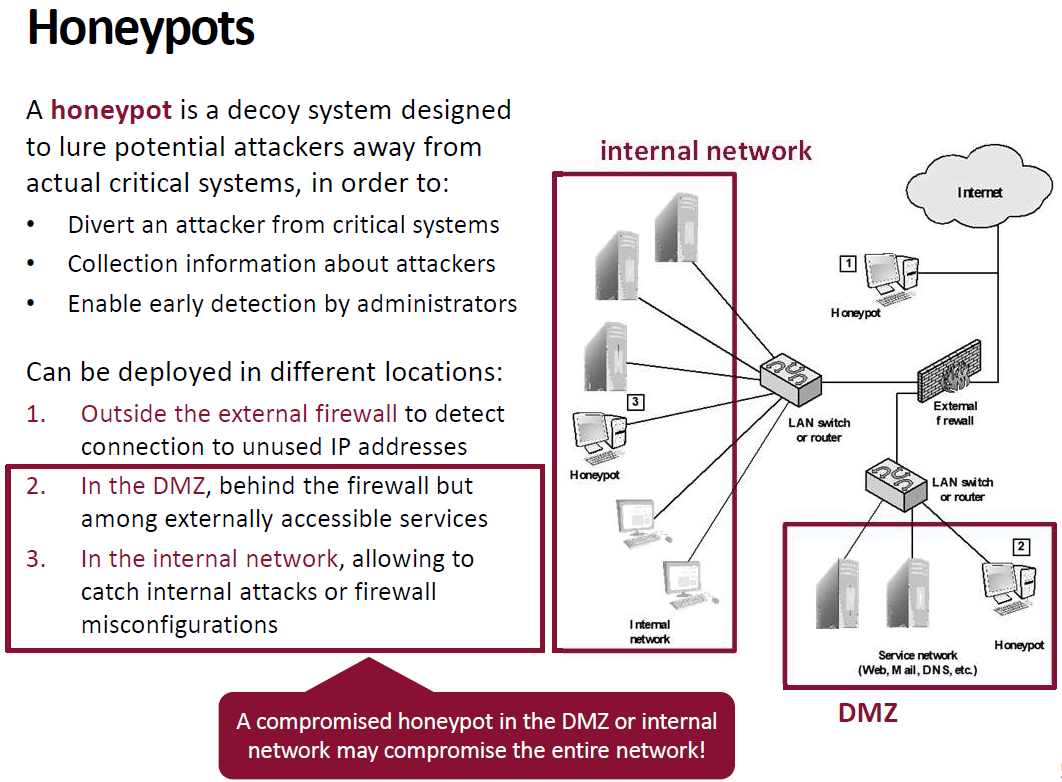
\includegraphics[width=\linewidth]{./slides/L6P4HONEY.PNG}
 
 \subsection{IP Security (IPSec) and VPN}
 IPSec encompasses 3 functional areas:
 \begin{itemize}
 	\item Authentication: assures that a received packet was in fact transmitted by the party identified as the source in the packet header.
 	\item Confidentiality: enables communicating nodes to encrypt messages to prevent eavesdropping by third parties.
 	\item Key management: secure exchange of keys.
 \end{itemize}
 
 \subsubsection{Modes of operation}
 \begin{enumerate}
 	\item Transport mode: provides protection primarily for upper-layer protocols $\rightarrow$ transport mode protection extends to payload of an IP packet, source and dest IP are not kept confidential, used for end-to-end communication between two hosts.\\
 	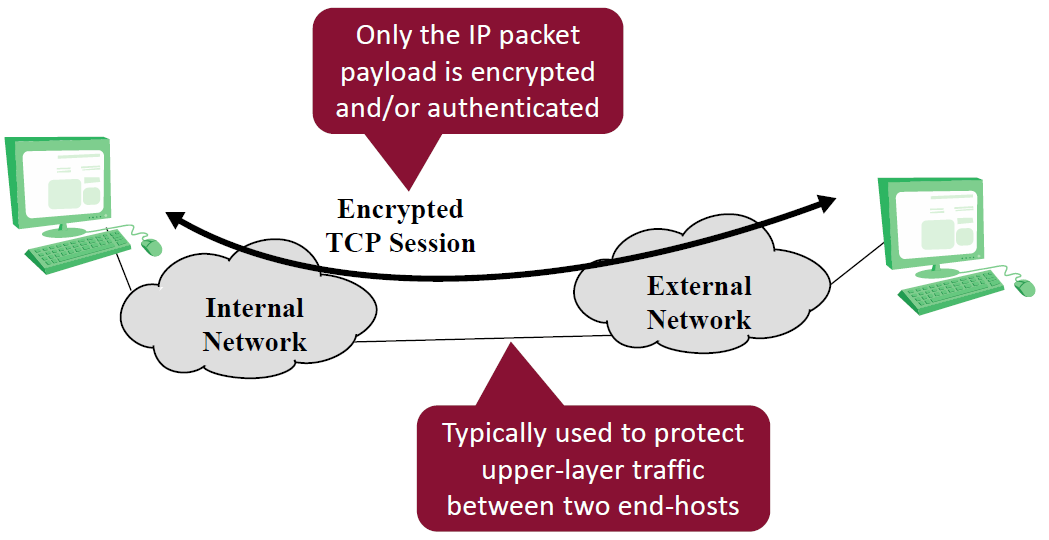
\includegraphics[width=0.8\linewidth]{./slides/L6P5MOD1.PNG}
 	\item Tunnel mode: provides protection to entire IP packet. After the AH er ESP fields are added to the IP packet, the entire packet plus security fields is treated as the payload of new outer IP packet with a new outer IP header. Used when one or both ends of a security association (SA) are a security gateway, such as a firewall or a router that implements IPSec.\\
 	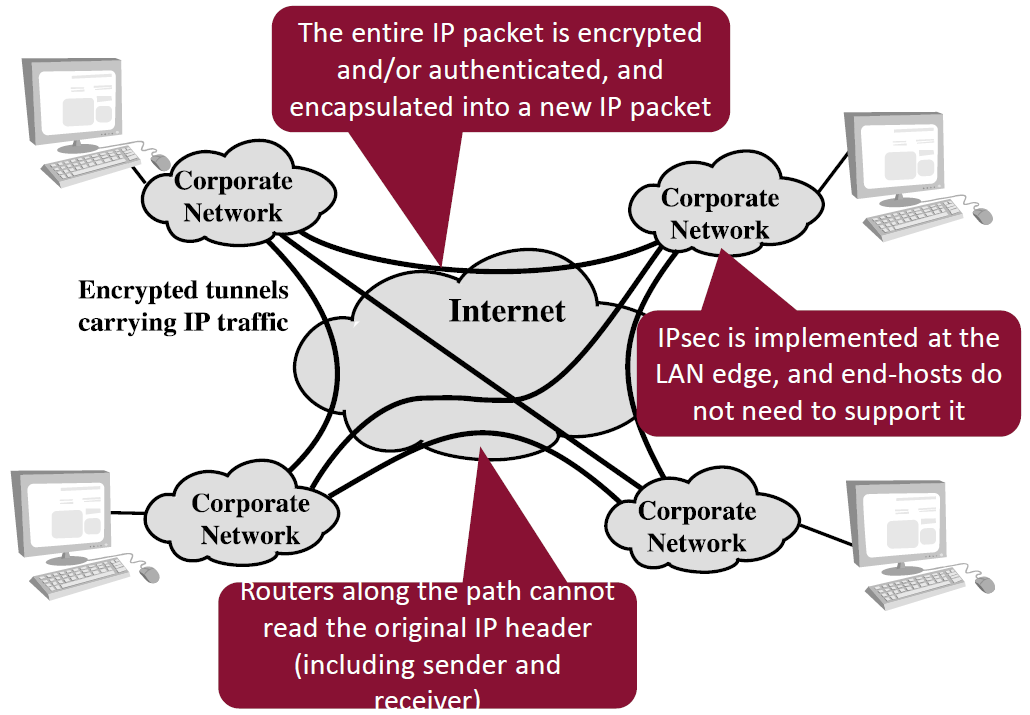
\includegraphics[width=0.8\linewidth]{./slides/L6P5MOD2.png}
 \end{enumerate}
 
 \subsubsection{IPSec architecture}
 IPSec is based on concept of a security policy applied to each IP packet that transits from source to dest. Policy is determined primarily by interaction of 2 DBs: security association DB (SAD) and security policy DB (SPD).\\
 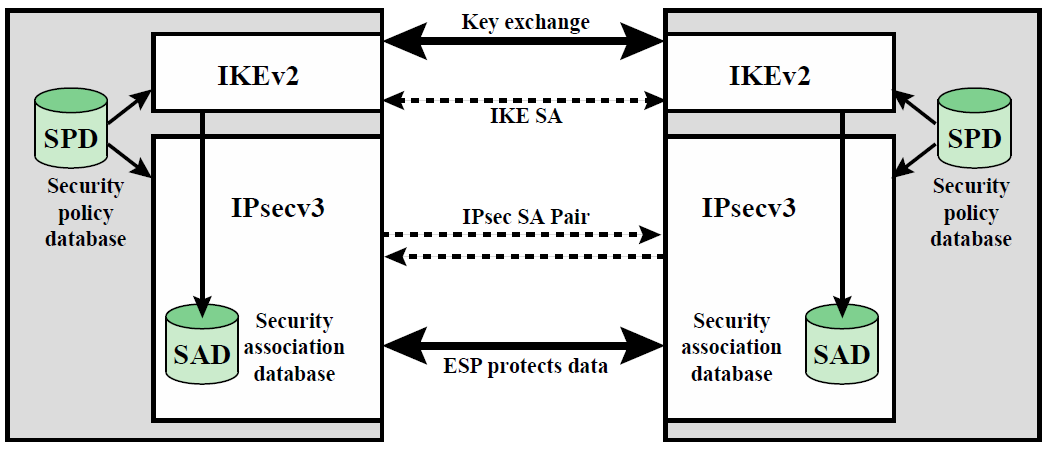
\includegraphics[width=\linewidth]{./slides/L6P5IPSECARCH.PNG}\\
 In each IPsec implementation, there is a nominal \textbf{Security Association Database (SAD) that defines the parameters associated with each SA}. The key management mechanism that is used to distribute keys is coupled to the authentication and privacy mechanisms only by way of the \textbf{Security Parameters Index (SPI)}. Hence, authentication and privacy have been specified independent of any specific key management mechanism.\\
 The \textbf{means by which IP traffic is related to specific SAs is the} nominal \textbf{Security Policy Database (SPD)}. In its simplest form, an SPD contains entries, each of which defines a subset of IP traffic and points to an SA for that traffic. In more complex environments, there may be multiple entries that potentially relate to a single SA or multiple SAs associated with a single SPD entry. \textbf{Each SPD entry is defined by a set of IP and upper-layer protocol field values, called selectors. In effect, these selectors are used to filter outgoing traffic in order to map it into a particular SA.} Possible selectors include: remote IP address, local IP address, next layer protocol, local port, and remote port.\\
 IPsec is executed on a packet-by-packet basis. When IPsec is implemented, each outbound IP packet is processed by the IPsec logic before transmission, and each inbound packet is processed by the IPsec logic after reception and before passing the packet contents on to the next higher layer (e.g., TCP or UDP).
 
 \subsubsection{Encapsulating Security payload (ESP)}
 One of two alternative security mechanisms in IPSec, ESP provides confidentiality and optionally authentication. The alternative Authentication Header (AH) only provides authentication. ESP can be used in combination with a wide range of encryption and authentication algorithms. \\
 Security services include packet confidentiality, data origin authentication, connection-less integrity, anti-replay service, (limited) traffic flow confidentiality.\\
 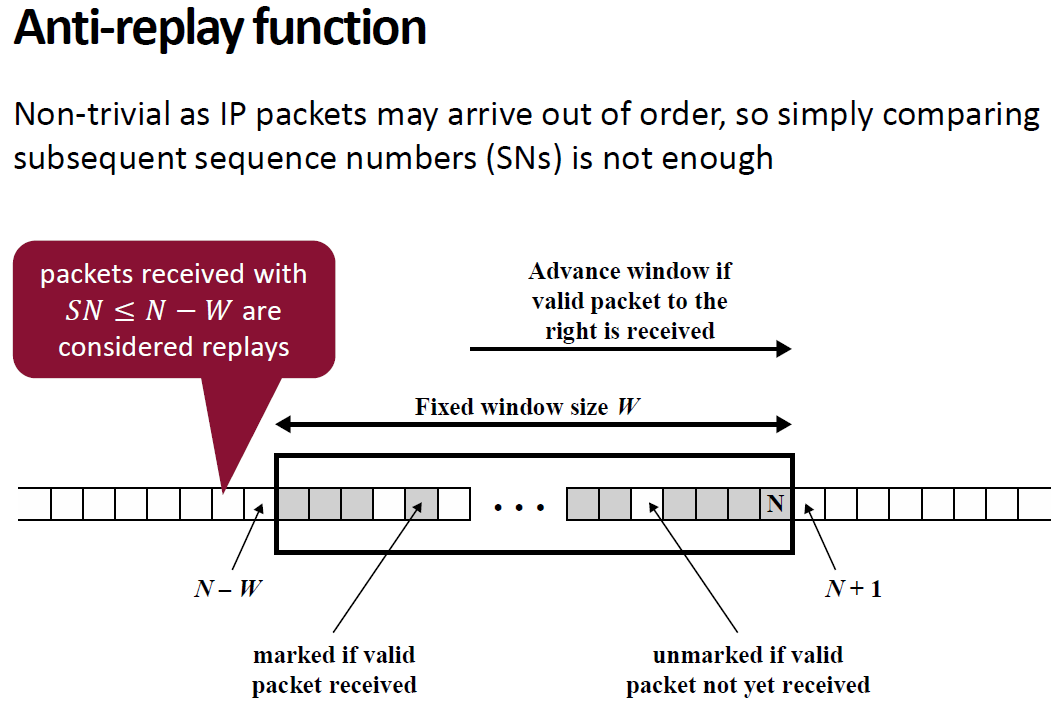
\includegraphics[width=0.8\linewidth]{./slides/L6P5ARF.PNG}
 
 \subsubsection{Internet key exchange}
 Goal: determination and distribution of secret keys for confidentiality and integrity.
 \begin{itemize}
 	\item Key exchange methods:
 	\begin{itemize}
 		\item Manual: sysadmin manually configures each system with the keys.
 		\item Automated: on demand creation of keys for SAs.
 	\end{itemize}
 \item Default automated key exchange methods:
 \begin{itemize}
 	\item Internet Security Association and Key Management Protocol: protocol for the negotiation of security attributes.
 	\item Oakley: key exchange protocol based on Diffie-Hellman.
 \end{itemize}
 \end{itemize}
  
 \newpage
 \section{Secure Network Protocols}
 
 \subsection{Wifi security basics}
 Wireless networks, and the wireless devices that use them, introduce a host of  security problems over and above those found in wired networks. Some of the key factors contributing to the higher security risk of wireless networks compared to wired networks include the following:
 \begin{itemize}
 	\item Channel: Wireless networking typically involves broadcast communications, which is far more susceptible to eavesdropping and jamming than wired networks. Wireless networks are also more vulnerable to active attacks that exploit vulnerabilities in communications protocols.
 	\item Mobility: Wireless devices are, in principal and usually in practice, far more portable and mobile than wired devices.
 	\item Resources: Some wireless devices, such as smartphones and tablets, have sophisticated operating systems but limited memory and processing resources with which to counter threats, including denial of service and malware.
 	\item Accessibility: Some wireless devices, such as sensors and robots, may be left unattended in remote and/or hostile locations. This greatly increases their	vulnerability to physical attacks.
 \end{itemize}
 Security threats to wireless networks:
 \begin{itemize}
 	\item Accidental association: Company wireless LANs or wireless access points to wired LANs in close proximity (e.g., in the same or neighboring buildings) may create overlapping transmission ranges. A user intending to connect to one LAN may	unintentionally lock on to a wireless access point from a neighboring network.
 	\item Malicious association: In this situation, a wireless device is configured to appear to be a legitimate access point, enabling the operator to steal passwords from legitimate users and then penetrate a wired network through a legitimate wireless access point.
 	\item Ad hoc networks: These are peer-to-peer networks between wireless computers with no access point between them. Such networks can pose a security threat due to a lack of a central point of control.
 	\item Nontraditional networks: Nontraditional networks and links, such as personal network Bluetooth devices, barcode readers, and handheld PDAs, pose a security risk in terms of both eavesdropping and spoofing.
 	\item Identity theft (MAC spoofing): This occurs when an attacker is able to eavesdrop on network traffic and identify the MAC address of a computer with network privileges.
 	\item Man-in-the middle attacks: This attack involves persuading a user and an access point to believe that they are talking to each other when in fact the communication is going through an intermediate attacking device. Wireless networks are particularly vulnerable to such attacks.
 	\item Denial of service (DoS): In the context of a wireless network, a DoS attack occurs when an attacker continually bombards a wireless access point or some other accessible wireless port with various protocol messages designed to consume system resources. The wireless environment lends itself to this type of attack,
 	because it is so easy for the attacker to direct multiple wireless messages at the target.
 	\item Network injection: A network injection attack targets wireless access points that are exposed to nonfiltered network traffic, such as routing protocol messages or network management messages. An example of such an attack is one in which bogus reconfiguration commands are used to affect routers and switches to
 	degrade network performance.
 \end{itemize}
 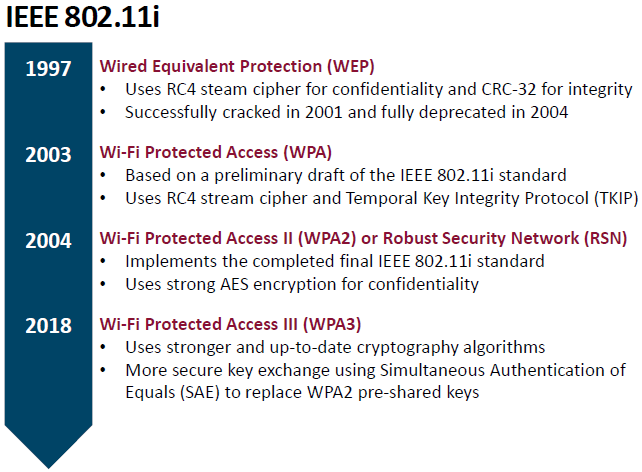
\includegraphics[width=\linewidth]{./slides/L7P1WIFIENCR.PNG}\footnote{WEP sucks, WPA is outdated}\\
 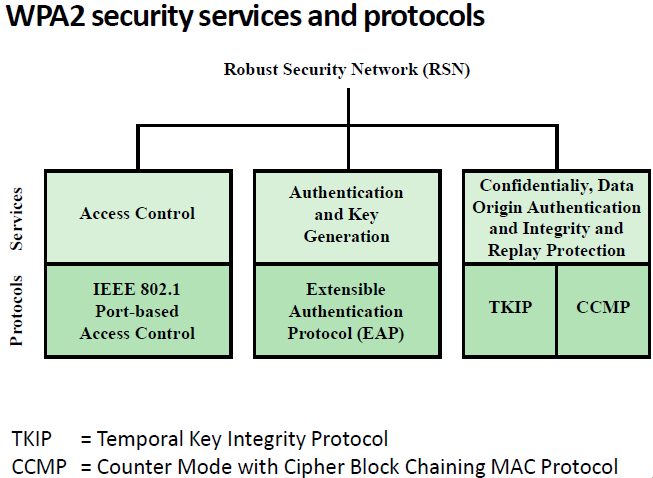
\includegraphics[width=\linewidth]{./slides/L7P1WPA2.PNG}\\
 The 802.11i RSN security specification defines the following services:
 \begin{itemize}
 	\item Authentication: A protocol is used to define an exchange between a user and an AS	that provides mutual authentication and generates temporary keys to be used between the client and the AP over the wireless link.
 	\item Access control: This function enforces the use of the authentication function, routes the messages properly, and facilitates key exchange. It can work with a variety of authentication protocols.
 	\item Privacy with message integrity: MAC-level data (e.g., an LLC PDU) are encrypted along with a message integrity code that ensures that the data have not been altered.
 \end{itemize}
 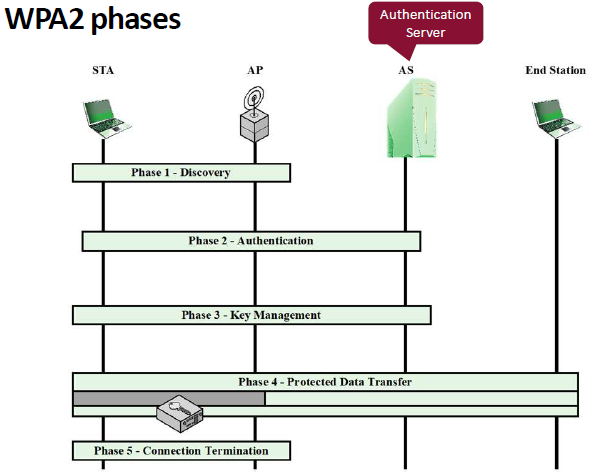
\includegraphics[width=\linewidth]{./slides/L7P1WPA2PH.PNG}\\
 The five phases are
 defined as follows:
 \begin{enumerate}
 	\item Discovery: An AP uses messages called Beacons and Probe Responses to advertise its IEEE 802.11i security policy. The STA uses these to identify an AP for a WLAN with which it wishes to communicate. The STA associates with the AP, which it uses to select the cipher suite and authentication mechanism when the Beacons and
 	Probe Responses present a choice. The discovery phase consists of three exchanges:
 	\begin{itemize}
 		\item Network and security capability discovery: During this exchange, STAs discover the existence of a network with which to communicate. The AP either periodically broadcasts its security capabilities (not shown in figure), indicated by RSN IE (Robust Security Network Information Element), in a specific channel through the Beacon frame; or responds to a station’s Probe Request through a Probe Response frame. A 	wireless station may discover available access points and corresponding security capabilities by either passively monitoring the Beacon frames or actively probing every channel.
 		\item Open system authentication: The purpose of this frame sequence, which provides no security, is simply to maintain backward compatibility with the IEEE 802.11 state machine, as implemented in existing IEEE 802.11 hardware. In essence, the two devices (STA and AP) simply exchange identifiers.
 		\item Association: The purpose of this stage is to agree on a set of security capabilities to be used. The STA then sends an Association Request frame to the AP. In this frame, the STA specifies one set of matching capabilities (one authentication and key management suite, one pairwise cipher suite, and one group-key cipher suite) from among those advertised by the AP. If there is no match in capabilities between the AP and the STA, the AP refuses the Association Request. The STA blocks it too, in case it has associated with a rogue AP or someone is inserting frames illicitly on its channel.
 	\end{itemize}
 	\item Authentication: During this phase, the STA and AS prove their identities to each other. The AP blocks non-authentication traffic between the STA and AS until the authentication transaction is successful. The AP does not participate in the authentication transaction other than forwarding traffic between the STA and AS. We can think of authentication phase as consisting of the following three phases:
 	\begin{itemize}
 		\item Connect to AS: The STA sends a request to its AP (the one with which it has an association) for connection to the AS. The AP acknowledges this request and sends an access request to the AS.
 		\item EAP exchange: This exchange authenticates the STA and AS to each other. A number of alternative exchanges are possible, as explained subsequently.
 		\item Secure key delivery: Once authentication is established, the AS generates a master session key (MSK), also known as the Authentication, Authorization, and Accounting (AAA) key and sends it to the STA. As explained subsequently, all the cryptographic keys needed by the STA for secure communication with its AP are generated from this MSK. IEEE 802.11i does not prescribe a method for secure delivery of the MSK but relies on EAP for this. Whatever method is used, it involves the transmission of an MPDU containing an encrypted MSK from the AS, via the AP, to the AS.
 	\end{itemize}
 	\item Key generation and distribution: The AP and the STA perform several operations that cause cryptographic keys to be generated and placed on the AP and the STA. Frames are exchanged between the AP and STA only.\\
 	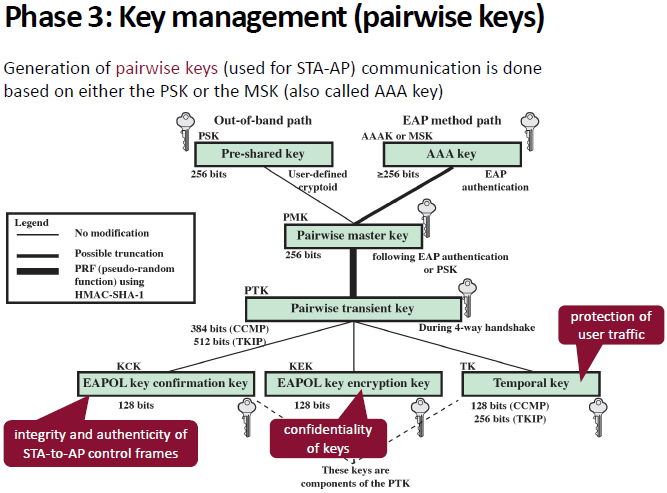
\includegraphics[width=\linewidth]{./slides/L7P1WPA2PH31.png}\\
 	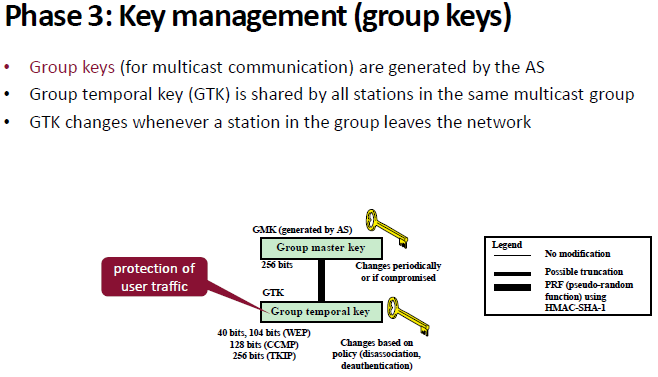
\includegraphics[width=\linewidth]{./slides/L7P1WPA2PH32.PNG}\\
 	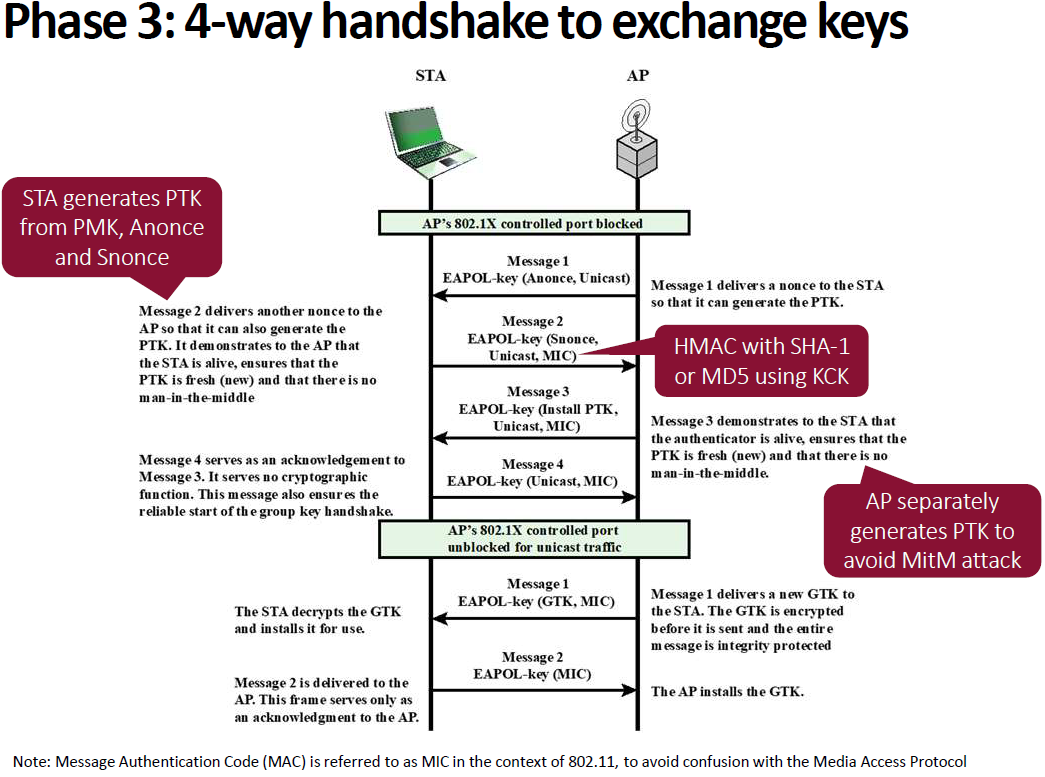
\includegraphics[width=\linewidth]{./slides/L7P1WPA2PH33.PNG}
 	\item Protected data transfer: Frames are exchanged between the STA and the end station through the AP. As denoted by the shading and the encryption module icon, secure data transfer occurs between the STA and the AP only; security is not provided end-to-end.\\
    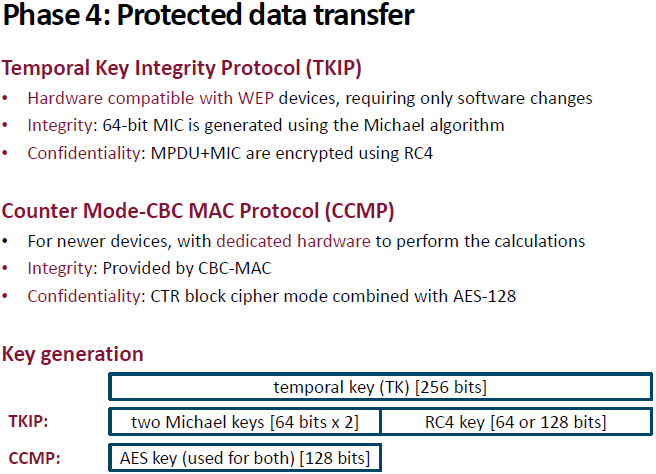
\includegraphics[width=\linewidth]{./slides/L7P1WPA2PH4.PNG}
 	\item Connection termination: The AP and STA exchange frames. During this phase, the secure connection is torn down and the connection is restored to the original state.
 \end{enumerate}
 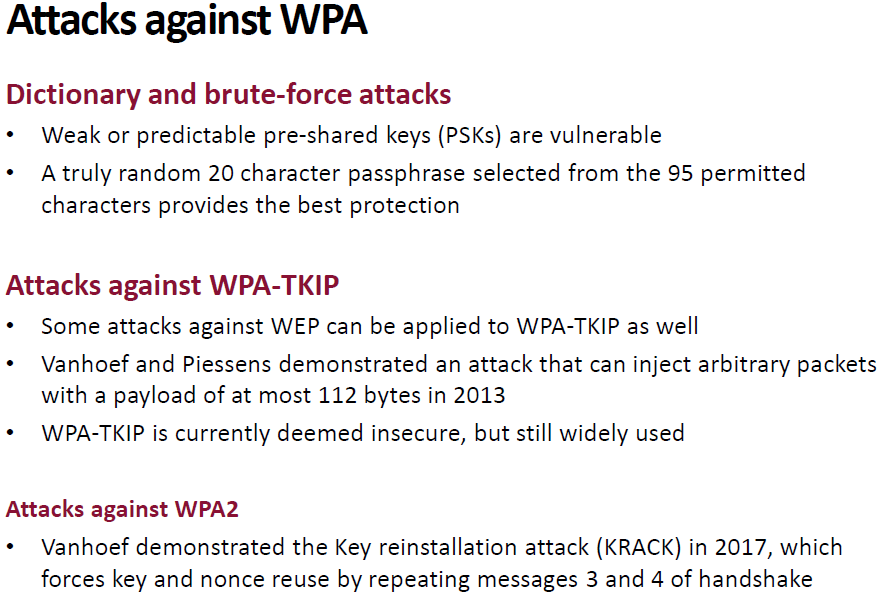
\includegraphics[width=\linewidth]{./slides/L7P1ATT.PNG}\\
 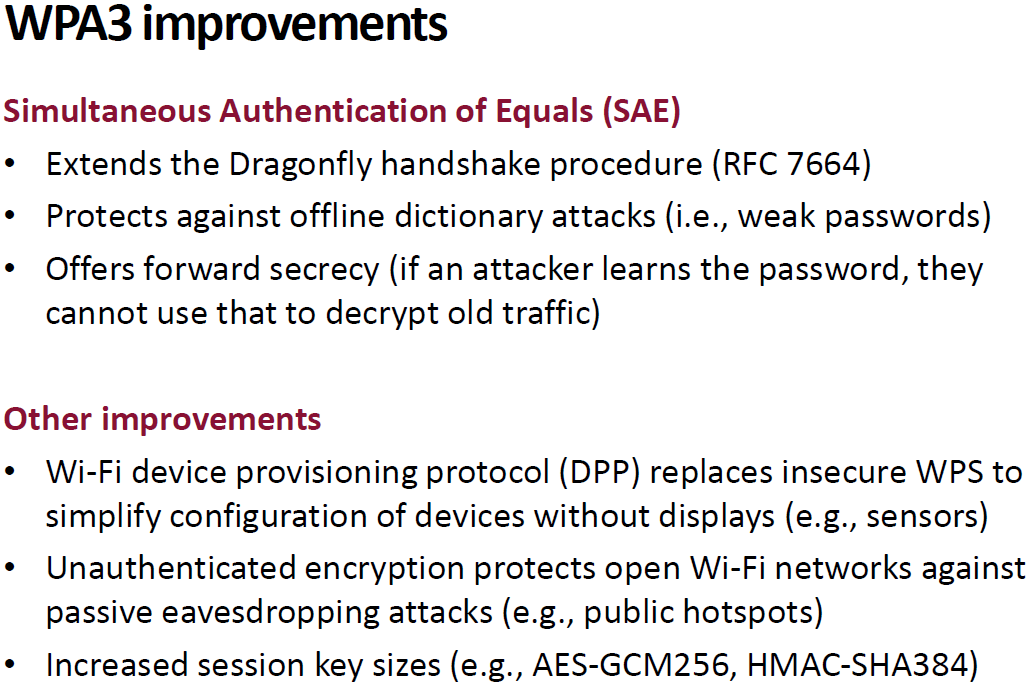
\includegraphics[width=\linewidth]{./slides/L7P1WPA3.PNG}
 
 \subsection{Transport layer security (SSL/TLS)}
 Two important TLS concepts are the TLS session and the TLS connection, which are defined in the specification as follows:
 \begin{itemize}
 	\item Connection: A connection is a transport that provides a suitable type of service. For TLS, such connections are peer-to-peer relationships. The connections are transient and every connection is associated with one session.
 	\item Session: A TLS session is an association between a client and a server and is created by the Handshake Protocol. Sessions define a set of cryptographic security parameters, which can be shared among multiple connections. Sessions are used to avoid the expensive negotiation of new security parameters for each connection.
 \end{itemize}
 TLS is designed to make use of TCP to provide a reliable end-to-end secure service. \textbf{TLS is not a single protocol but rather two layers of protocols}. The \textbf{TLS Record Protocol} provides basic security services to various higher-layer protocols. In particular, the Hypertext Transfer Protocol (HTTP), which provides the transfer service for Web client/server interaction,\textbf{ can operate on top of TLS}. \textbf{Three higher-layer protocols are defined as part of TLS:} the Handshake Protocol; the Change Cipher Spec Protocol; and the Alert Protocol. These TLS-specific protocols are used in the management of TLS exchanges and are examined later. A fourth protocol, the Heartbeat Protocol, is defined in a separate RFC and is also discussed subsequently.\\
 The TLS Record Protocol provides two services for TLS connections:
 \begin{itemize}
 	\item Confidentiality: The Handshake Protocol defines a shared secret key that is used for conventional encryption of TLS payloads.
 	\item Message Integrity: The Handshake Protocol also defines a shared secret key that is used to form a message authentication code (MAC).
 \end{itemize}
 The Record Protocol takes an application message to be transmitted, fragments the data into manageable blocks, optionally compresses the data, applies a MAC, encrypts, adds a header, and transmits the resulting unit in a TCP segment. Received data are decrypted, verified, decompressed, and reassembled before being delivered to higherlevel
 users.\\
 The first step is fragmentation. Each upper-layer message is fragmented into blocks of  $2^{14}$ bytes or less. Next, compression is optionally applied. Compression must be lossless and may not increase the content length by more than 1024 bytes. In TLSv2, no compression algorithm is specified, so the default compression algorithm is
 null. The next step in processing is to compute a message authentication code over the compressed data.\\
 Next, the compressed message plus the MAC are encrypted using symmetric encryption. Encryption may not increase the content length by more than 1024 bytes, so that the total length may not exceed 214 + 2048. For stream encryption, the compressed message plus the MAC are encrypted. For block encryption, padding may be added after the MAC prior to encryption. The padding is in the form of a number of padding bytes followed by a one-byte indication of the length of the padding.\\
 The final step of TLS Record Protocol processing is to prepend a header consisting of the following fields:
 \begin{itemize}
 	\item Content Type (8 bits): The higher-layer protocol used to process the enclosed fragment.
 	\item Major Version (8 bits): Indicates major version of TLS in use. For TLSv2, the value is 3.
 	\item Minor Version (8 bits): Indicates minor version in use. For TLSv2, the value is 1.
 	\item Compressed Length (16 bits): The length in bytes of the fragment. The maximum value is 214 + 2048.
 \end{itemize}
 \subsubsection{Handshake protocol phases} 
 The Handshake protocol consist of 4 phases.\\
 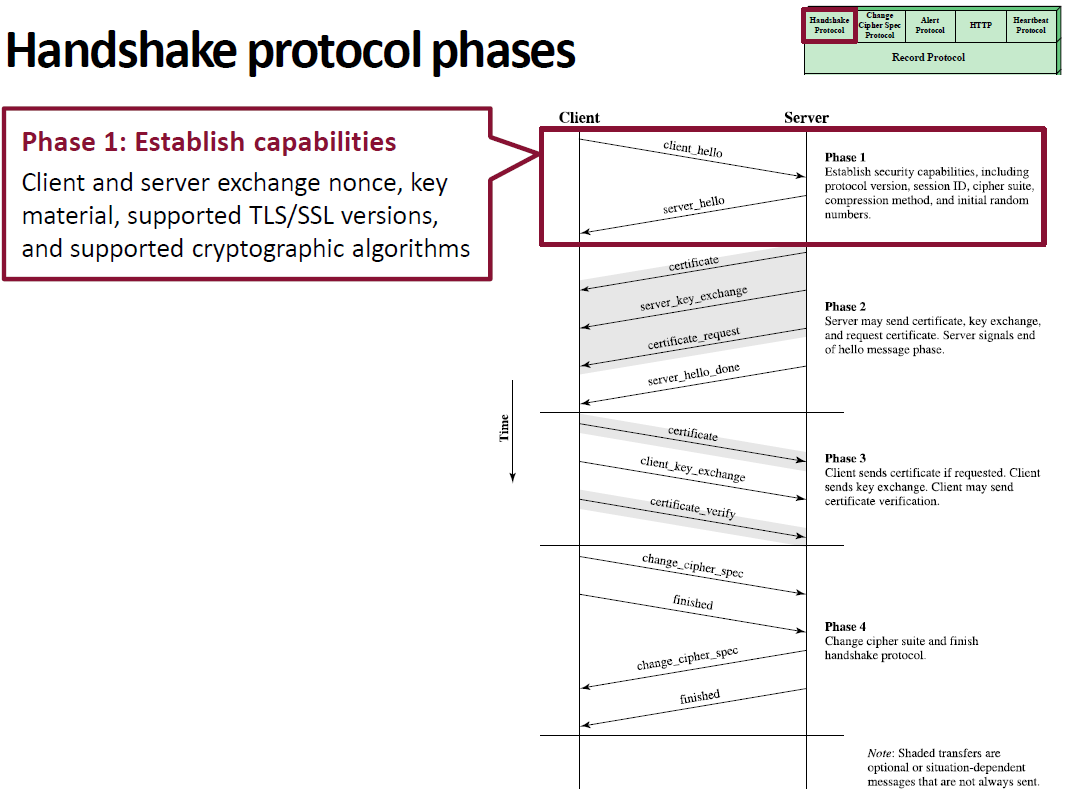
\includegraphics[width=\linewidth]{./slides/L7P2HSP1.png}\\
 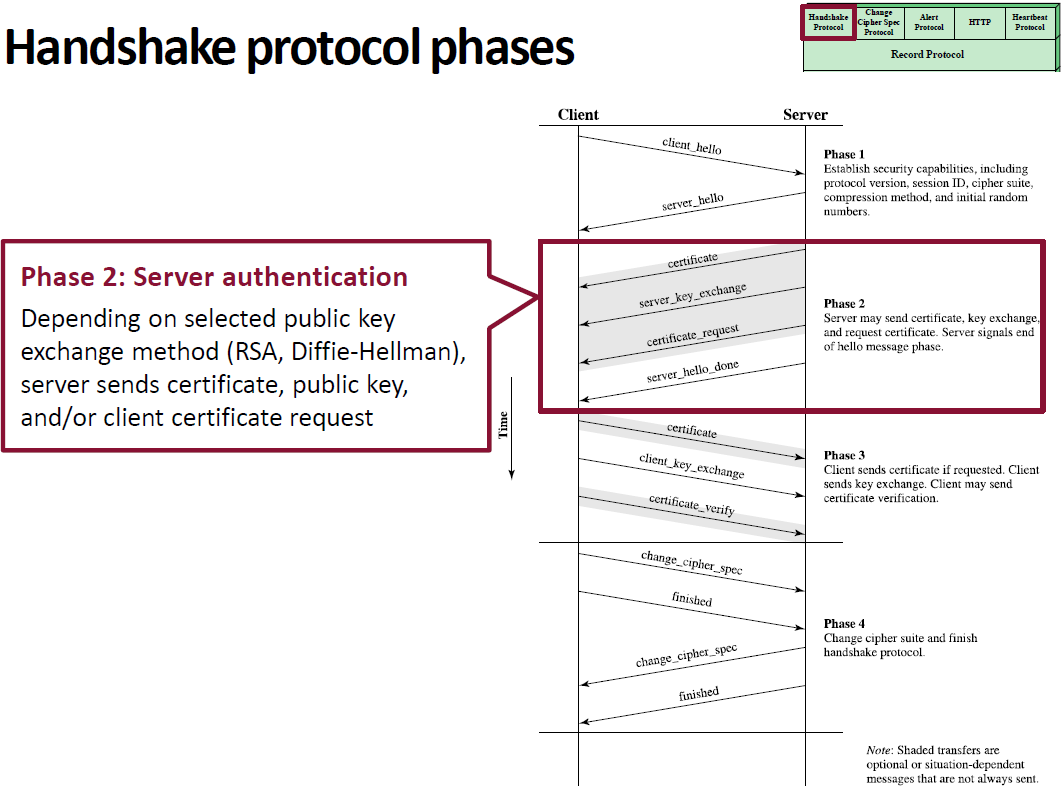
\includegraphics[width=\linewidth]{./slides/L7P2HSP2.png}\\
 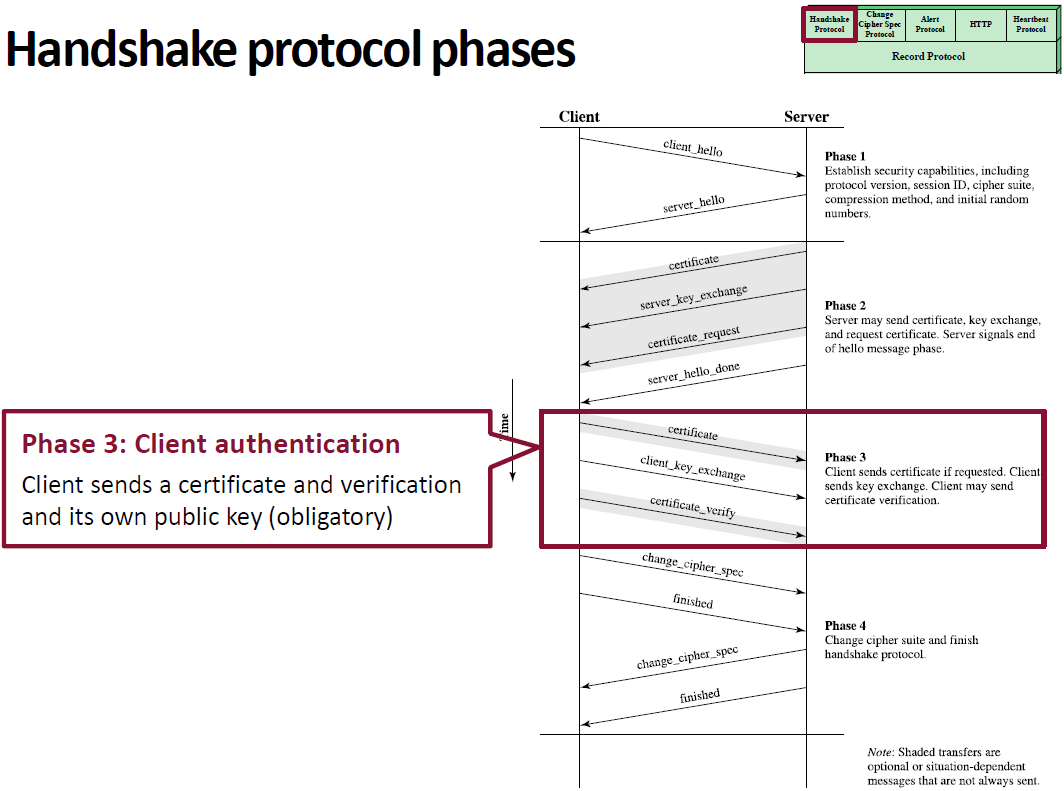
\includegraphics[width=\linewidth]{./slides/L7P2HSP3.png}\\
 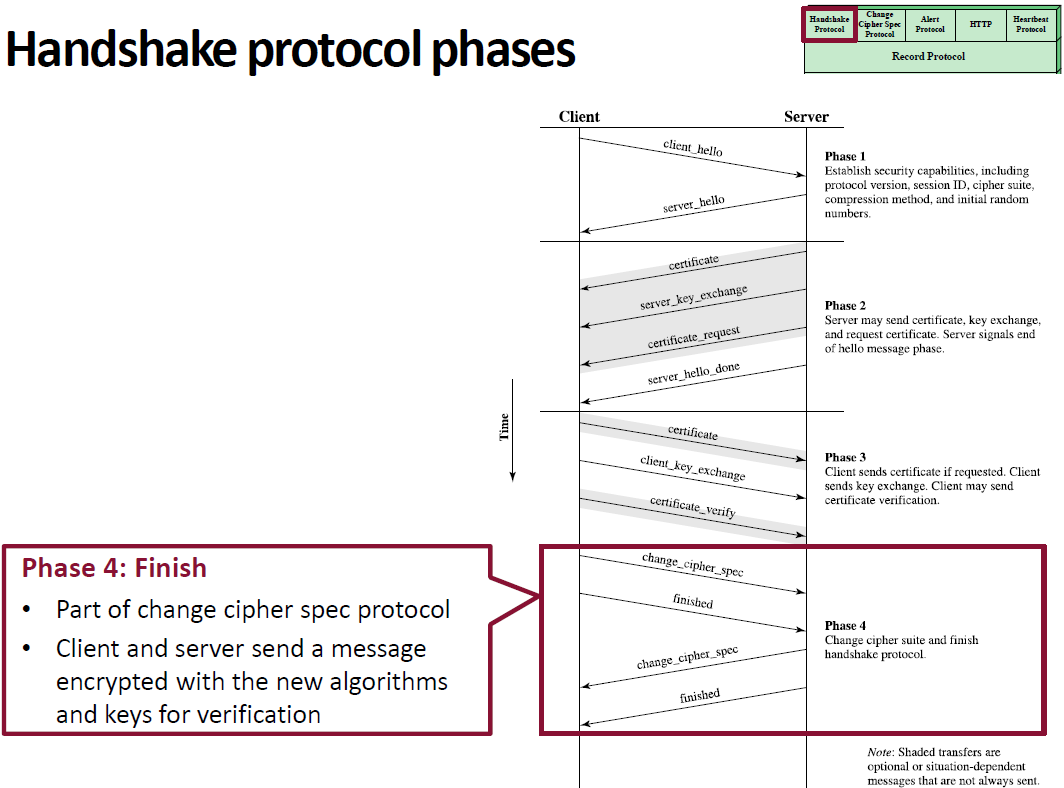
\includegraphics[width=\linewidth]{./slides/L7P2HSP4.png}
 
 \subsubsection{Creation of symmetric keys}
 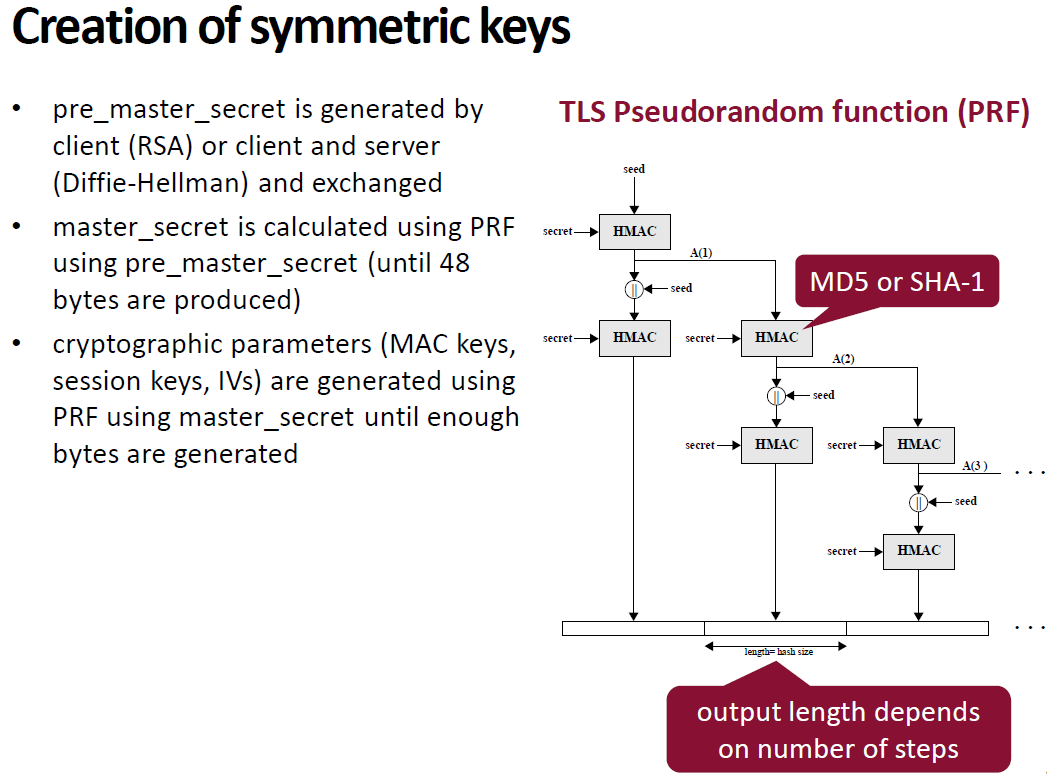
\includegraphics[width=\linewidth]{./slides/L7P2SYMK.PNG}\\
 The creation is in two stages. First, a pre\_master\_secret is exchanged. Second, the master\_secret is calculated by both parties. For pre\_master\_secret exchange, there are two possibilities: RSA of Diffie-Hellman.\\
 Both sides now compute the master\_secret as\\
 master\_secret = PRF(pre\_master\_secret, “master secret”, ClientHello.random $||$ ServerHello.random)\\
 where ClientHello.random and ServerHello.random are the two nonce values exchanged in the initial hello messages.\\
 The algorithm is performed until 48 bytes of pseudorandom output are produced. The calculation of the key block material (MAC secret keys, session encryption keys, and IVs) is defined as:\\
 key\_block = PRF(SecurityParameters.master\_secret, “key expansion”, SecurityParameters.server\_random $||$ SecurityParameters.client\_random)\\
 until enough output has been generated.\\
 CipherSpecs require a client write MAC secret, a server write MAC secret, a client write key, a server write key, a client write IV, and a server write IV, which are generated from the master secret in that order. These parameters are generated from the master secret by hashing the master secret into a sequence of secure bytes of sufficient length for all needed parameters.\\
 The generation of the key material from the master secret uses the same format for generation of the master secret from the pre-master secret as\\
 \texttt{key\_block =\\ 
 	MD5(master\_secret $||$ SHA(‘A’ $||$ master\_secret $||$ ServerHello.random $||$ ClientHello.random)) $||$ \\
 	MD5(master\_secret $||$ SHA(‘BB’ $||$ master\_secret $||$ ServerHello.random $||$ ClientHello.random)) $||$\\
 	MD5(master\_secret $||$ SHA(‘CCC’ $||$ master\_secret $||$ ServerHello.random $||$ ClientHello.random)) $||$\\
 	...}\\
 until enough output has been generated. The result of this algorithmic structure is a pseudorandom function. We can view the master\_secret as the pseudorandom seed value to the function. The client and server random numbers can be viewed as salt values to complicate cryptanalysis.\\
 TLS makes use of a pseudorandom function referred to as PRF to expand secrets into blocks of data for purposes of key generation or validation. The objective is to make use of a relatively small, shared secret value but to generate longer blocks of data in a way that is secure from the kinds of attacks made on hash functions and MACs. The data expansion function makes use of the HMAC algorithm with either MD5 or SHA-1 as the underlying hash function.
 
 \subsection{Attacks against SSL and TLS}
 \subsubsection{Heartbleed attack}
 Caused by a minor programming error in the OpenSSL implementation: \texttt{memcpy(bp, pl, payloadsize)}. If \texttt{pl} array is smaller than what \texttt{payloadsize} makes believe, old data in memory alloted to \texttt{bp} array is not overwritten and returned to the attacker.\\
 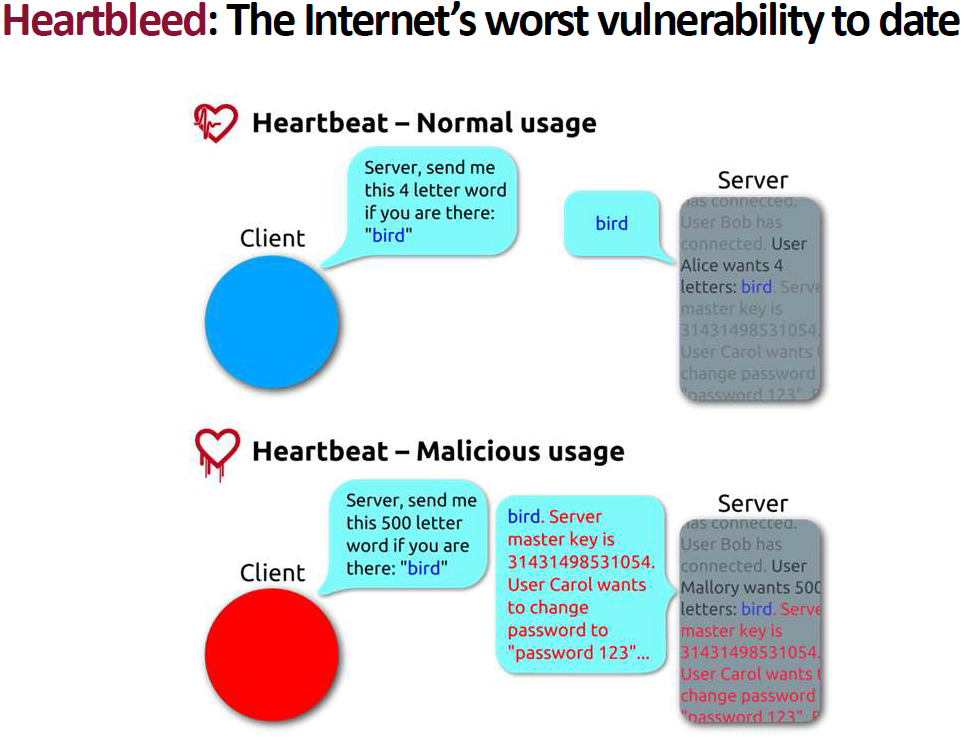
\includegraphics[width=\linewidth]{./slides/L7P3HBA.PNG}\\
 \includegraphics[width=\linewidth]{./slides/L7P3HBAF.PNG}
 
 \subsubsection{POODLE}
 POODLE is an attack against TLS.\\
 \includegraphics[width=\linewidth]{./slides/L7P3POODLE.PNG}\\
 \includegraphics[width=\linewidth]{./slides/L7P3PAD.PNG}\\
 \includegraphics[width=0.8\linewidth]{./slides/L7P3PADONE.PNG}\\
 \includegraphics[width=0.8\linewidth]{./slides/L7P3PADPREV.PNG}
 
 \subsection{Secure SHell}
 Secure Shell (SSH) is a protocol for secure network communications designed to be relatively simple and inexpensive to implement, it is used for both secure remote logon facilities and network functions as file transfer and email.\\
 \includegraphics[width=\linewidth]{./slides/L7P4SSHSTACK.PNG}\\
 If you want details on the handshake protocol, do go to the slides (it's too much and too detailed for here).\\
 \includegraphics[width=0.8\linewidth]{./slides/L7P4SSHPACK.png}\\
 \includegraphics[width=0.8\linewidth]{./slides/L7P4SSHAUTH.PNG}\\
 \includegraphics[width=0.8\linewidth]{./slides/L7P4SSHCON.PNG}\\
 \includegraphics[width=0.8\linewidth]{./slides/L7P4SSHPORT.PNG}\\
 Port forwarding: traffic is intercepted on the local host (client)/remote host (server) and forwarded to the given host and port via the remote host (server)/local host (client). \\
 Command: \texttt{ssh <-L/-R> x:remotehost:y user@sshserver}
 
 \newpage
 \section{Application layer security}
 \subsection{Email security}
 \includegraphics[width=1.2\linewidth]{./slides/L8P1THR.PNG}\\
 \includegraphics[width=0.8\linewidth]{./slides/L8P1MECH.PNG}\\
 \subsubsection{SMIME}
 \includegraphics[width=0.8\linewidth]{./slides/L8P1SMIME.PNG}\\
 \includegraphics[width=0.9\linewidth]{./slides/L8P1sSMIME.PNG}
 \subsubsection{PGP}
 An alternative email security protocol is Pretty Good Privacy (PGP), which has essentially the same functionality as S/MIME. The actual operation of PGP, as opposed to the management of keys, consists of four services: authentication, confidentiality, compression, and e-mail compatibility.\\
 Both authentication and confidentiality services may be used for the same message. First, a signature is generated for the plaintext message and prepended to the message. Then the plaintext message plus signature is encrypted using CAST-128 (or IDEA or 3DES), and the session key is encrypted using RSA (or ElGamal). When both services are used, the sender first signs the message with its own private key, then encrypts the message with a session key,
 and finally encrypts the session key with the recipient’s public key.\\
 As a default, PGP compresses the message after applying the signature but before encryption. This has the benefit of saving space both for e-mail transmission and for file storage.\\
 The signature is generated before compression for two reasons:
 \begin{enumerate}
 	\item It is preferable to sign an uncompressed message so that one can store only the uncompressed message together with the signature for future verification. If one signed a compressed document, then it would be necessary either to store a compressed version of the message for later verification or to recompress the message when verification is required.
 	\item Even if one were willing to generate dynamically a recompressed message for verification, PGP’s compression algorithm presents a difficulty. The algorithm is not deterministic; various implementations of the algorithm achieve different tradeoffs in running speed versus compression ratio and, as a result, produce different compressed forms. However, these different compression algorithms are interoperable because any version of the algorithm can correctly decompress the output of any other version. Applying the hash function and signature after compression would constrain all PGP implementations to the same version of the compression algorithm.
 \end{enumerate}
 Message encryption is applied after compression to strengthen cryptographic security. Because the compressed message has less redundancy than the original plaintext, cryptanalysis is more difficult.\\
 \includegraphics[width=0.9\linewidth]{./slides/L8P1PGPK.PNG}\\
 \includegraphics[width=\linewidth]{./slides/L8P1COMP.PNG}
 
 \subsection{Web security}
 The Open Web Application Security Project (OWASP) is a 501(c)(3) worldwide not-forprofit charitable organization focused on improving the security of software. OWASP is in a unique position to provide impartial, practical
 information about AppSec to individuals, corporations, universities, government agencies and other organizations worldwide. Operating as a community of like-minded professionals, OWASP issues software tools and knowledge-based documentation on application security.\\
 OWASP top 10 web application vulnerabilities:
 \begin{enumerate}
 	\item Injection: Injection flaws, such as SQL, NoSQL, OS, and LDAP injection, occur when untrusted data is
 	sent to an interpreter as part of a command or query. The attacker's hostile data can trick	the interpreter into executing unintended commands or accessing data without proper	authorization.
 	\item Broken Authentication: Application functions related to authentication and session management are often
 	implemented incorrectly, allowing attackers to compromise passwords, keys, or session tokens, or to exploit other implementation flaws to assume other users' identities temporarily or permanently.
 	\item Sensitive Data Exposure: Many web applications and APIs do not properly protect sensitive data, such as financial, healthcare, and PII. Attackers may steal or modify such weakly protected data to conduct credit card fraud, identity theft, or other crimes. Sensitive data may be compromised without extra protection, such as encryption at rest or in transit, and requires special precautions when exchanged with the browser.
 	\item XML External Entities (XXE): Many older or poorly configured XML processors evaluate external entity references within XML documents. External entities can be used to disclose internal files using the file URI handler, internal file shares, internal port scanning, remote code execution, and denial of service attacks.
 	\item Broken Access Control: Restrictions on what authenticated users are allowed to do are often not properly
 	enforced. Attackers can exploit these flaws to access unauthorized functionality and/or data, such as access other users' accounts, view sensitive files, modify other users' data, change access rights, etc.
 	\item Security Misconfiguration: Security misconfiguration is the most commonly seen issue. This is commonly a result of insecure default configurations, incomplete or ad hoc configurations, open cloud storage, misconfigured HTTP headers, and verbose error messages containing sensitive information. Not only must all operating systems, frameworks, libraries, and applications be securely configured, but they must be patched/upgraded in a timely fashion.
 	\item Cross-Site Scripting (XSS): XSS flaws occur whenever an application includes untrusted data in a new web page without proper validation or escaping, or updates an existing web page with usersupplied data using a browser API that can create HTML or JavaScript. XSS allows attackers to execute scripts in the victim's browser which can hijack user sessions, deface web sites, or redirect the user to malicious sites.
 	\item Insecure Deserialization: Insecure deserialization often leads to remote code execution. Even if deserialization flaws do not result in remote code execution, they can be used to perform attacks, including replay attacks, injection attacks, and privilege escalation attacks.
 	\item Using Components with Known Vulnerabilities: Components, such as libraries, frameworks, and other software modules, run with the same privileges as the application. If a vulnerable component is exploited, such an attack can facilitate serious data loss or server takeover. Applications and APIs using components
 	with known vulnerabilities may undermine application defenses and enable various attacks and impacts.
 	\item Insufficient Logging \& Monitoring: Insufficient logging and monitoring, coupled with missing or ineffective integration with incident response, allows attackers to further attack systems, maintain persistence, pivot to more systems, and tamper, extract, or destroy data. Most breach studies show time to detect a breach is over 200 days, typically detected by external parties rather than internal processes or monitoring.
 \end{enumerate}
 \includegraphics[width=0.9\linewidth]{./slides/L8P2SQL.PNG}\\
 \includegraphics[width=0.9\linewidth]{./slides/L8P2XXE.PNG}\\
 \includegraphics[width=0.9\linewidth]{./slides/L8P2XSS.PNG}\\
 \includegraphics[width=0.9\linewidth]{./slides/L8P2XSSPREV.PNG}
 
 \subsection{Malicious software}
 \includegraphics[width=\linewidth]{./slides/L8P3MWT.png}
 \subsubsection{Trojan horse browser: Zeus-in-the-mobile (ZitMo)}
 Mobile ZeuS, or Trojan-Spy.*.Zitmo, was designed for one sole purpose: to quickly steal mTAN\footnote{mobile transaction authentication numbers} codes without mobile users noticing. The user attempts to navigate to  his bank’s webpage and log into the system. The PC version of ZeuS registers that the victim is going to an address of interest, and modifies this webpage in the browser so that the personal data entered by the user for authentication is not sent to the bank, but to the ZeuS botnet command center. A modified authentication page would also ask the user to enter data about their mobile device (the make, model, and telephone number) in addition to their username and password. Users were told that the data was requested for the alleged purpose of certificate updates. Sooner or later, users who provided information to malicious users about their cell phones would receive a text messages asking them to install a new security certificate. This “security certificate” could be downloaded via a link that was provided in the text message. However, this “certificate” was in fact the mobile version of the ZeuS Trojan. Then his mobile phone would be infected by ZitMo, the primary function of which is to send a text message to a malicious user’s phone as specified in the body of the Trojan.\\
 The malicious users who successfully used the PC-based ZeuS to steal personal user data for online banking systems and infect victims’ phones with ZitMo were thus able to overcome the last barrier of online banking security systems: the mTAN code. By entering a user’s login and password, they were able to access their bank accounts and conduct transactions (such as transferring money from the user’s account to their own bank accounts). These transactions required additional authentication using a code sent by the bank via text message to the client’s phone.\\
 After the client submitted a transaction request, the bank would send the client an authentication code. The code would be sent to the ZitMo-infected handset, which immediately forwarded it to the malicious user’s number, who would then use the stolen mTAN to authenticate the transaction. And the victim would be none the wiser.\\
 The attacks are generally orchestrated as follows:
 \begin{enumerate}
 	\item Cyber criminals use the PC-based ZeuS to steal the data needed to access online banking accounts and client cell phone numbers.
 	\item The victim’s mobile phone (see point 1) receives a text message with a request to install an updated security certificate, or some other necessary software. However, the link in the text message will actually lead to the mobile version of ZeuS.
 	\item If the victim installs this software and infects the phone, the malicious user can then use the stolen personal data and attempt to make cash transactions from the compromised account, but still needs an mTAN code to authenticate the transaction.
 	\item The bank sends out a text message with the mTAN code to the client’s mobile phone. ZitMo forwards the text message with the mTAN code to the malicious user’s phone. The malicious user is then able to use the mTAN code to authenticate the transaction.
 \end{enumerate}
 \subsubsection{Malware propagation}
 \includegraphics[width=\linewidth]{./slides/L8P3MWP.PNG}\\
 The first category of malware propagation concerns parasitic software fragments that attach themselves to some existing executable content. The fragment may be machine code that infects some existing application, utility, or system program, or even the code used to boot a computer system.\\
 A worm is a program that actively seeks out more machines to infect, and then each infected machine serves as an automated launching pad for attacks on other machines. Worm programs exploit software vulnerabilities in client or server programs to gain access to each new system. They can use network connections to spread from system to system.\\
 The final category of malware propagation we consider involves social engineering, “tricking” users to assist in the compromise of their own systems or personal information. This can occur when a user views and responds to some SPAM e-mail or permits the installation and execution of some Trojan horse program or scripting code.
 \subsubsection{Malware payload}
 \includegraphics[width=\linewidth]{./slides/L8P3MWPL.PNG}\\
 An early payload seen in a number of viruses and worms resulted in data destruction on the infected system when certain trigger conditions were met. A related payload is one that displays unwanted messages or content on the user’s system when triggered. More seriously, another variant attempts to inflict realworld damage on the system. All of these actions target the integrity of the computer system’s software or hardware, or of the user’s data. These changes may not occur immediately, but only when specific trigger conditions are met that satisfy their logic-bomb code. As an alternative to just destroying data, some malware encrypts the user’s data and demands payment in order to access the key needed to recover this information. This is sometimes known as ransomware.\\
 The next category of payload we discuss is where the malware subverts the computational and network resources of the infected system for use by the attacker. Such a system is known as a bot (robot), zombie, or drone, and secretly takes over another Internet-attached computer and then uses that computer to launch or manage attacks that are difficult to trace to the bot’s creator. The bot is typically planted on hundreds or thousands of computers belonging to unsuspecting third parties. The collection of bots often is capable of acting in a coordinated manner; such a collection is referred to as a botnet. This type of payload attacks the integrity and availability of the infected system.\\
 We now consider payloads where the malware gathers data stored on the infected system for use by the attacker. A common target is the user’s login and password credentials to banking, gaming, and related sites, which the attacker then uses to impersonate the user to access these sites for gain. Less commonly, the payload may target documents or system configuration details for the purpose of reconnaissance or espionage. These attacks target the confidentiality of this information.\\
 The final category of payload we discuss concerns techniques used by malware to hide its presence on the infected system and to provide covert access to that system. This type of payload also attacks the integrity of the infected system.
 \subsubsection{DDoS}
 A denial-of-service (DoS) attack is an attempt to prevent legitimate users of a service from using that service. When this attack comes from a single host or network node, then it is simply referred to as a DoS attack. A more serious threat is posed by a DDoS attack. DDoS attacks make computer systems inaccessible by flooding servers, networks, or even end-user systems with useless traffic so that legitimate users can no longer gain access to those resources. In a typical DDoS attack, a large number of compromised hosts are amassed to send useless packets.\\
 A DDoS attack attempts to consume the target’s resources so that it cannot provide service. One way to classify DDoS attacks is in terms of the type of resource that is consumed. Broadly speaking, the resource consumed is either an internal host resource on the target system or data transmission capacity in the local network to which the target is attacked.\\
 \includegraphics[width=0.9\linewidth]{./slides/L8P3DDOSSYN.PNG}\\
 \includegraphics[width=0.9\linewidth]{./slides/L8P3DDOSICMP.png}
 
 \section{Guest lecture: IoT}
 \subsection{Introduction}
 Security challenges in IoT:
 \begin{enumerate}
 	\item Rapid Proliferation of IoT Devices\\
 	One of the biggest IoT security challenges is keeping up with the production of IoT connected devices. The concern is not that the IoT devices are increasing each day. The issue is that these devices are not protected. Most small and medium-sized businesses continue to connect several unprotected objects, such as smart lighting,
 	barcode readers, smart locks, security cameras, and HVAC systems to their IT networks.
 	\item It is Hard to Protect What You Can’t See\\
 	Hackers are proactively looking for new techniques to penetrate IoT devices, so organizations should always find vulnerabilities and fix them as soon as they occur. Predicting and preventing these threats is even more desirable. However, the primary attack vector is usually the invisibility of networks. The fact that most enterprises can’t detect devices on their system means that they won’t protect what they cannot see.
 	\item Default Passwords and Brute-Forcing\\
 	Many manufacturers supply consumers with products that have default login information, such as the username and passwords. This information is what cybercriminals are looking for to carry out a brute-force attack on the affected devices. The Mirai botnet serves as an example of the issues that come with selling devices with default credentials and not informing the consumers to change them. The most worrying thing is that most of the default passwords are painfully obvious, such that even an ordinary user can guess them. So, with inadequate out-of-the-box security features, consumers ought to take security measures into their own hands.
 	\item Lack of Proper Testing and Updating\\
 	As the need for connected devices increases, more manufacturers are working hard to produce new ones. The only challenge is that they do not pay enough attention to security. Most of these devices rarely get updates. Sometimes, they don’t even get updates at all. What it means is that these devices are only secure at the time of purchase, but remain open to attacks once hackers find security loopholes. In other words, if no one fixes the security issues on time, for both software and hardware, these products remain vulnerable to attacks.
 	\item Increased Attacks Targeting IoT Devices\\
 	As the IoT technology continues to advance, so does the complexity of attacks. In fact, IoT devices were one of the main cyberattack vectors in 2018. It seems the more interconnected devices we have, the more interesting it gets for the attackers, which calls for the industry to come up with more effective security initiatives. Fortunately, most of the security vulnerabilities in 2020 will be the ones known to IT security professionals. Organizations should, therefore, stay focused on fixing the risks they already know. It could be as simple as installing the right Windows error solutions with malware protection capabilities.
 	\item Data Privacy and Security\\
 	In today’s interconnected world, data privacy and security are becoming increasingly challenging. The main issue is that data gets transferred between multiple devices. At one moment, it may be stored on a computer, and the next moment it is on the web or the cloud. As you know, not all devices or platforms that transmit data are secure. It gets worse when you consider that the information goes through the internet, which could leak it out to criminals. Organizations should design privacy and compliance rules that anonymize personal information before storing it. They should then apply this practice to the web, mobile, and cloud applications, including services that are used to access and process data on IoT devices.
 	\item Poorly Encrypted Communications\\
 	Encryption is one of the great ways to keep attackers away from accessing crucial data. Unfortunately, it is also one of the leading IoT security challenges. Currently, most devices lack process and storage capabilities found in standard computers. What this means is that cybercriminals can easily manipulate the algorithms that are supposed to protect the devices. If no one addresses the issue, then encryption won’t help much.
 	\item Larger and More Frequent IoT Botnets Targeting Cryptomining\\
 	A botnet can access data, send spam, and allow access to devices without users’ knowledge. An example of such attacks is the 2016 Mirai, a botnet powered by over 60 login credentials. The recent rise in currency valuation, coupled with the ongoing mining spree, would make it too attractive for attackers, trying to benefit from the crypto-craze. The Blockchain framework is usually resistant to hacking, but there have been successful
 	attempts to penetrate the system and extract usernames and passwords. Actually, the main vulnerability is the Blockchain app development, and not the Blockchain itself. So, IoT botnets and Blockchain breaches will continue to pose a high risk to IoT structures, applications, and platforms that rely on Blockchain technology.
 	\item IoT Automation Challenges\\
 	As IoT devices continue to make way into our lives, organizations will reach a point where they will be dealing with thousands or even millions of devices at once. Obviously, it would be difficult for anyone to manage the massive amount of data produced by these interconnected devices, especially from networking and data 	collection perspectives. Network and IoT admins will, therefore, need to use AI tools to automate data 	management. However, the use of these tools to handle big data can pose a security threat if not managed well. A minor misconfiguration of AI tools can trigger an outage.
 	\item Unauthorized Home Access\\
 	Perhaps one of the places where we might feel the impact of IoT the most is in our homes. Today, most developers fit new buildings with IoT devices. While this might be a good thing, it can also be a security concern. Not everyone is knowledgeable about the best practices that should be maintained about IoT security. Some IoT devices you use at home can expose your IP address, thus revealing your residential address. Anyone who has access to this information can use it to carry out criminal activities.
 \end{enumerate}
 
\end{document}







